%% bare_jrnl_compsoc.tex
%% V1.3
%% 2007/01/11
%% by Michael Shell
%% See:
%% http://www.michaelshell.org/
%% for current contact information.
%%
%% This is a skeleton file demonstrating the use of IEEEtran.cls
%% (requires IEEEtran.cls version 1.7 or later) with an IEEE Computer
%% Society journal paper.
%%
%% Support sites:
%% http://www.michaelshell.org/tex/ieeetran/
%% http://www.ctan.org/tex-archive/macros/latex/contrib/IEEEtran/
%% and
%% http://www.ieee.org/

%%*************************************************************************
%% Legal Notice:
%% This code is offered as-is without any warranty either expressed or
%% implied; without even the implied warranty of MERCHANTABILITY or
%% FITNESS FOR A PARTICULAR PURPOSE!
%% User assumes all risk.
%% In no event shall IEEE or any contributor to this code be liable for
%% any damages or losses, including, but not limited to, incidental,
%% consequential, or any other damages, resulting from the use or misuse
%% of any information contained here.
%%
%% All comments are the opinions of their respective authors and are not
%% necessarily endorsed by the IEEE.
%%
%% This work is distributed under the LaTeX Project Public License (LPPL)
%% ( http://www.latex-project.org/ ) version 1.3, and may be freely used,
%% distributed and modified. A copy of the LPPL, version 1.3, is included
%% in the base LaTeX documentation of all distributions of LaTeX released
%% 2003/12/01 or later.
%% Retain all contribution notices and credits.
%% ** Modified files should be clearly indicated as such, including  **
%% ** renaming them and changing author support contact information. **
%%
%% File list of work: IEEEtran.cls, IEEEtran_HOWTO.pdf, bare_adv.tex,
%%                    bare_conf.tex, bare_jrnl.tex, bare_jrnl_compsoc.tex
%%*************************************************************************

% *** Authors should verify (and, if needed, correct) their LaTeX system  ***
% *** with the testflow diagnostic prior to trusting their LaTeX platform ***
% *** with production work. IEEE's font choices can trigger bugs that do  ***
% *** not appear when using other class files.                            ***
% The testflow support page is at:
% http://www.michaelshell.org/tex/testflow/




% Note that the a4paper option is mainly intended so that authors in
% countries using A4 can easily print to A4 and see how their paper's will
% look in print - the typesetting of the document will not typically be
% affected with changes in paper size (but the bottom and side margins will).
% Use the testflow package mentioned above to verify correct handling of
% both paper sizes by the user's LaTeX system.
%
% Also note that the "draftcls" or "draftclsnofoot", not "draft", option
% should be used if it is desired that the figures are to be displayed in
% draft mode.
%
% The Computer Society usually requires 10pt for submissions.
%
\documentclass[10pt,journal,letterpaper,twoside]{IEEEtran}
%
% If IEEEtran.cls has not been installed into the LaTeX system files,
% manually specify the path to it like:
% \documentclass[12pt,journal,compsoc]{../sty/IEEEtran}





% Some very useful LaTeX packages include:
% (uncomment the ones you want to load)


% *** MISC UTILITY PACKAGES ***
%
%\usepackage{ifpdf}
% Heiko Oberdiek's ifpdf.sty is very useful if you need conditional
% compilation based on whether the output is pdf or dvi.
% usage:
% \ifpdf
%   % pdf code
% \else
%   % dvi code
% \fi
% The latest version of ifpdf.sty can be obtained from:
% http://www.ctan.org/tex-archive/macros/latex/contrib/oberdiek/
% Also, note that IEEEtran.cls V1.7 and later provides a builtin
% \ifCLASSINFOpdf conditional that works the same way.
% When switching from latex to pdflatex and vice-versa, the compiler may
% have to be run twice to clear warning/error messages.






% *** CITATION PACKAGES ***
%
%\ifCLASSOPTIONcompsoc
  % IEEE Computer Society needs nocompress option
  % requires cite.sty v4.0 or later (November 2003)
  \usepackage[nocompress]{cite}
%\else
  % normal IEEE
  \usepackage{cite}
%\fi
% cite.sty was written by Donald Arseneau
% V1.6 and later of IEEEtran pre-defines the format of the cite.sty package
% \cite{} output to follow that of IEEE. Loading the cite package will
% result in citation numbers being automatically sorted and properly
% "compressed/ranged". e.g., [1], [9], [2], [7], [5], [6] without using
% cite.sty will become [1], [2], [5]--[7], [9] using cite.sty. cite.sty's
% \cite will automatically add leading space, if needed. Use cite.sty's
% noadjust option (cite.sty V3.8 and later) if you want to turn this off.
% cite.sty is already installed on most LaTeX systems. Be sure and use
% version 4.0 (2003-05-27) and later if using hyperref.sty. cite.sty does
% not currently provide for hyperlinked citations.
% The latest version can be obtained at:
% http://www.ctan.org/tex-archive/macros/latex/contrib/cite/
% The documentation is contained in the cite.sty file itself.
%
% Note that some packages require special options to format as the Computer
% Society requires. In particular, Computer Society  paper's do not use
% compressed citation ranges as is done in typical IEEE paper's
% (e.g., [1]-[4]). Instead, they list every citation separately in order
% (e.g., [1], [2], [3], [4]). To get the latter we need to load the cite
% package with the nocompress option which is supported by cite.sty v4.0
% and later. Note also the use of a CLASSOPTION conditional provided by
% IEEEtran.cls V1.7 and later.





% *** GRAPHICS RELATED PACKAGES ***
%
%\ifCLASSINFOpdf
  % \usepackage[pdftoeps]{graphicx}
  % declare the path(s) where your graphic files are
  % \graphicspath{{../pdf/}{../jpeg/}}
  % and their extensions so you won't have to specify these with
  % every instance of \includegraphics
  % \DeclareGraphicsExtensions{.pdf,.jpeg,.png}
%\else
  % or other class option (dvipsone, dvipdf, if not using dvips). graphicx
  % will default to the driver specified in the system graphics.cfg if no
  % driver is specified.
  \usepackage[dvips]{graphicx}
%  \usepackage{graphicx}
  \usepackage{float}
  % declare the path(s) where your graphic files are
  % \graphicspath{{../eps/}}
  % and their extensions so you won't have to specify these with
  % every instance of \includegraphics
  % \DeclareGraphicsExtensions{.eps}
%\fi
% graphicx was written by David Carlisle and Sebastian Rahtz. It is
% required if you want graphics, photos, etc. graphicx.sty is already
% installed on most LaTeX systems. The latest version and documentation can
% be obtained at:
% http://www.ctan.org/tex-archive/macros/latex/required/graphics/
% Another good source of documentation is "Using Imported Graphics in
% LaTeX2e" by Keith Reckdahl which can be found as epslatex.ps or
% epslatex.pdf at: http://www.ctan.org/tex-archive/info/
%
% latex, and pdflatex in dvi mode, support graphics in encapsulated
% postscript (.eps) format. pdflatex in pdf mode supports graphics
% in .pdf, .jpeg, .png and .mps (metapost) formats. Users should ensure
% that all non-photo figures use a vector format (.eps, .pdf, .mps) and
% not a bitmapped formats (.jpeg, .png). IEEE frowns on bitmapped formats
% which can result in "jaggedy"/blurry rendering of lines and letters as
% well as large increases in file sizes.
%
% You can find documentation about the pdfTeX application at:
% http://www.tug.org/applications/pdftex





% *** MATH PACKAGES ***
%
\let\latexvec=\vec
\usepackage[cmex10]{amsmath}
\usepackage{amssymb}
\let\vec=\latexvec
% A popular package from the American Mathematical Society that provides
% many useful and powerful commands for dealing with mathematics. If using
% it, be sure to load this package with the cmex10 option to ensure that
% only type 1 fonts will utilized at all point sizes. Without this option,
% it is possible that some math symbols, particularly those within
% footnotes, will be rendered in bitmap form which will result in a
% document that can not be IEEE Xplore compliant!
%
% Also, note that the amsmath package sets \interdisplaylinepenalty to 10000
% thus preventing page breaks from occurring within multiline equations. Use:
\interdisplaylinepenalty=2500
% after loading amsmath to restore such page breaks as IEEEtran.cls normally
% does. amsmath.sty is already installed on most LaTeX systems. The latest
% version and documentation can be obtained at:
% http://www.ctan.org/tex-archive/macros/latex/required/amslatex/math/





% *** SPECIALIZED LIST PACKAGES ***
%
\usepackage{algpseudocode}
\renewcommand{\algorithmicrequire}{\textbf{Input:}}
\renewcommand{\algorithmicensure}{\textbf{Output:}}
% \usepackage{algorithmic}
% algorithmic.sty was written by Peter Williams and Rogerio Brito.
% This package provides an algorithmic environment for describing algorithms.
% You can use the algorithmic environment in-text or within a figure
% environment to provide for a floating algorithm. Do NOT use the algorithm
% floating environment provided by algorithm.sty (by the same authors) or
% algorithm2e.sty (by Christophe Fiorio) as IEEE does not use dedicated
% algorithm float types and packages that provide these will not provide
% correct IEEE style captions. The latest version and documentation of
% algorithmic.sty can be obtained at:
% http://www.ctan.org/tex-archive/macros/latex/contrib/algorithms/
% There is also a support site at:
% http://algorithms.berlios.de/index.html
% Also of interest may be the (relatively newer and more customizable)
% algorithmicx.sty package by Szasz Janos:
% http://www.ctan.org/tex-archive/macros/latex/contrib/algorithmicx/




% *** ALIGNMENT PACKAGES ***
%
\usepackage{array}
% Frank Mittelbach's and David Carlisle's array.sty patches and improves
% the standard LaTeX2e array and tabular environments to provide better
% appearance and additional user controls. As the default LaTeX2e table
% generation code is lacking to the point of almost being broken with
% respect to the quality of the end results, all users are strongly
% advised to use an enhanced (at the very least that provided by array.sty)
% set of table tools. array.sty is already installed on most systems. The
% latest version and documentation can be obtained at:
% http://www.ctan.org/tex-archive/macros/latex/required/tools/


%\usepackage{mdwmath}
%\usepackage{mdwtab}
% Also highly recommended is Mark Wooding's extremely powerful MDW tools,
% especially mdwmath.sty and mdwtab.sty which are used to format equations
% and tables, respectively. The MDWtools set is already installed on most
% LaTeX systems. The lastest version and documentation is available at:
% http://www.ctan.org/tex-archive/macros/latex/contrib/mdwtools/


% IEEEtran contains the IEEEeqnarray family of commands that can be used to
% generate multiline equations as well as matrices, tables, etc., of high
% quality.


% \usepackage{eqparbox}
% Also of notable interest is Scott Pakin's eqparbox package for creating
% (automatically sized) equal width boxes - aka "natural width parboxes".
% Available at:
% http://www.ctan.org/tex-archive/macros/latex/contrib/eqparbox/





% *** SUBFIGURE PACKAGES ***
% \ifCLASSOPTIONcompsoc
 \usepackage[tight,normalsize,sf,SF]{subfigure}
% \else
% \usepackage[tight,footnotesize]{subfigure}
% \fi
% subfigure.sty was written by Steven Douglas Cochran. This package makes it
% easy to put subfigures in your figures. e.g., "Figure 1a and 1b". For IEEE
% work, it is a good idea to load it with the tight package option to reduce
% the amount of white space around the subfigures. Computer Society paper's
% use a larger font and \sffamily font for their captions, hence the
% additional options needed under compsoc mode. subfigure.sty is already
% installed on most LaTeX systems. The latest version and documentation can
% be obtained at:
% http://www.ctan.org/tex-archive/obsolete/macros/latex/contrib/subfigure/
% subfigure.sty has been superceeded by subfig.sty.


%\ifCLASSOPTIONcompsoc
%  \usepackage[caption=false]{caption}
%  \usepackage[font=normalsize,labelfont=sf,textfont=sf]{subfig}
%\else
%  \usepackage[caption=false]{caption}
%  \usepackage[font=footnotesize]{subfig}
%\fi
% subfig.sty, also written by Steven Douglas Cochran, is the modern
% replacement for subfigure.sty. However, subfig.sty requires and
% automatically loads Axel Sommerfeldt's caption.sty which will override
% IEEEtran.cls handling of captions and this will result in nonIEEE style
% figure/table captions. To prevent this problem, be sure and preload
% caption.sty with its "caption=false" package option. This is will preserve
% IEEEtran.cls handing of captions. Version 1.3 (2005/06/28) and later
% (recommended due to many improvements over 1.2) of subfig.sty supports
% the caption=false option directly:
%\ifCLASSOPTIONcompsoc
%  \usepackage[caption=false,font=normalsize,labelfont=sf,textfont=sf]{subfig}
%\else
  \usepackage[caption=false,font=footnotesize]{subfig}
%\fi
%
% The latest version and documentation can be obtained at:
% http://www.ctan.org/tex-archive/macros/latex/contrib/subfig/
% The latest version and documentation of caption.sty can be obtained at:
% http://www.ctan.org/tex-archive/macros/latex/contrib/caption/




% *** FLOAT PACKAGES ***
%
\usepackage{fixltx2e}
\usepackage{float}
% fixltx2e, the successor to the earlier fix2col.sty, was written by
% Frank Mittelbach and David Carlisle. This package corrects a few problems
% in the LaTeX2e kernel, the most notable of which is that in current
% LaTeX2e releases, the ordering of single and double column floats is not
% guaranteed to be preserved. Thus, an unpatched LaTeX2e can allow a
% single column figure to be placed prior to an earlier double column
% figure. The latest version and documentation can be found at:
% http://www.ctan.org/tex-archive/macros/latex/base/



%\usepackage{stfloats}
% stfloats.sty was written by Sigitas Tolusis. This package gives LaTeX2e
% the ability to do double column floats at the bottom of the page as well
% as the top. (e.g., "\begin{figure*}[!b]" is not normally possible in
% LaTeX2e). It also provides a command:
%\fnbelowfloat
% to enable the placement of footnotes below bottom floats (the standard
% LaTeX2e kernel puts them above bottom floats). This is an invasive package
% which rewrites many portions of the LaTeX2e float routines. It may not work
% with other packages that modify the LaTeX2e float routines. The latest
% version and documentation can be obtained at:
% http://www.ctan.org/tex-archive/macros/latex/contrib/sttools/
% Documentation is contained in the stfloats.sty comments as well as in the
% presfull.pdf file. Do not use the stfloats baselinefloat ability as IEEE
% does not allow \baselineskip to stretch. Authors submitting work to the
% IEEE should note that IEEE rarely uses double column equations and
% that authors should try to avoid such use. Do not be tempted to use the
% cuted.sty or midfloat.sty packages (also by Sigitas Tolusis) as IEEE does
% not format its paper's in such ways.




%\ifCLASSOPTIONcaptionsoff
%  \usepackage[nomarkers]{endfloat}
% \let\MYoriglatexcaption\caption
% \renewcommand{\caption}[2][\relax]{\MYoriglatexcaption[#2]{#2}}
%\fi
% endfloat.sty was written by James Darrell McCauley and Jeff Goldberg.
% This package may be useful when used in conjunction with IEEEtran.cls'
% captionsoff option. Some IEEE journals/societies require that submissions
% have lists of figures/tables at the end of the paper and that
% figures/tables without any captions are placed on a page by themselves at
% the end of the document. If needed, the draftcls IEEEtran class option or
% \CLASSINPUTbaselinestretch interface can be used to increase the line
% spacing as well. Be sure and use the nomarkers option of endfloat to
% prevent endfloat from "marking" where the figures would have been placed
% in the text. The two hack lines of code above are a slight modification of
% that suggested by in the endfloat docs (section 8.3.1) to ensure that
% the full captions always appear in the list of figures/tables - even if
% the user used the short optional argument of \caption[]{}.
% IEEE paper's do not typically make use of \caption[]'s optional argument,
% so this should not be an issue. A similar trick can be used to disable
% captions of packages such as subfig.sty that lack options to turn off
% the subcaptions:
% For subfig.sty:
% \let\MYorigsubfloat\subfloat
% \renewcommand{\subfloat}[2][\relax]{\MYorigsubfloat[]{#2}}
% For subfigure.sty:
% \let\MYorigsubfigure\subfigure
% \renewcommand{\subfigure}[2][\relax]{\MYorigsubfigure[]{#2}}
% However, the above trick will not work if both optional arguments of
% the \subfloat/subfig command are used. Furthermore, there needs to be a
% description of each subfigure *somewhere* and endfloat does not add
% subfigure captions to its list of figures. Thus, the best approach is to
% avoid the use of subfigure captions (many IEEE journals avoid them anyway)
% and instead reference/explain all the subfigures within the main caption.
% The latest version of endfloat.sty and its documentation can obtained at:
% http://www.ctan.org/tex-archive/macros/latex/contrib/endfloat/
%
% The IEEEtran \ifCLASSOPTIONcaptionsoff conditional can also be used
% later in the document, say, to conditionally put the References on a
% page by themselves.




% *** PDF, URL AND HYPERLINK PACKAGES ***
%
\usepackage{url}
% url.sty was written by Donald Arseneau. It provides better support for
% handling and breaking URLs. url.sty is already installed on most LaTeX
% systems. The latest version can be obtained at:
% http://www.ctan.org/tex-archive/macros/latex/contrib/misc/
% Read the url.sty source comments for usage information. Basically,
% \url{my_url_here}.


% Other packages
\usepackage{becs}

\usepackage{listings}
\lstset{%
  basicstyle=\scriptsize,
  numbers=left,
  numberstyle=\tiny,
  stepnumber=1,
  xleftmargin=2em
}

% Theorem-like environments
\newtheorem{definition}{Definition}
\newtheorem{exampleb}{Example}

% \subsubsubsection - really!?
\newcommand{\subsubsubsection}[1]{\medskip\par\emph{#1:}}
\newcommand{\swarmA}{Hexagonal}
\newcommand{\swarmB}{Connected}
\newcommand{\stability}{internal movement}
\newcommand{\Stability}{Internal movement}
\newcommand{\Fig}{fig.}
\newcommand{\Figs}{figs.}
\newcommand{\Eq}{eq.}
\newcommand{\Eqs}{eqs.}

% *** Do not adjust lengths that control margins, column widths, etc. ***
% *** Do not use packages that alter fonts (such as pslatex).         ***
% There should be no need to do such things with IEEEtran.cls V1.6 and later.
% (Unless specifically asked to do so by the journal or conference you plan
% to submit to, of course. )


% correct bad hyphenation here
\hyphenation{op-tical net-works semi-conduc-tor}

\begin{document}
%
% paper title
% can use linebreaks \\ within to get better formatting as desired
\title{Analysis of the \stability{} of mobile swarms}
%
%
% author names and IEEE memberships
% note positions of commas and nonbreaking spaces ( ~ ) LaTeX will not break
% a structure at a ~ so this keeps an author's name from being broken across
% two lines.
% use \thanks{} to gain access to the first footnote area
% a separate \thanks must be used for each paragraph as LaTeX2e's \thanks
% was not built to handle multiple paragraphs
%
%
%\IEEEcompsocitemizethanks is a special \thanks that produces the bulleted
% lists the Computer Society journals use for "first footnote" author
% affiliations. Use \IEEEcompsocthanksitem which works much like \item
% for each affiliation group. When not in compsoc mode,
% \IEEEcompsocitemizethanks becomes like \thanks and
% \IEEEcompsocthanksitem becomes a line break with idention. This
% facilitates dual compilation, although admittedly the differences in the
% desired content of \author between the different types of paper's makes a
% one-size-fits-all approach a daunting prospect. For instance, compsoc
% journal paper's have the author affiliations above the "Manuscript
% received ..."  text while in non-compsoc journals this is reversed. Sigh.

\author{Neil Eliot, David Kendall, Michael Brockway
\IEEEcompsocitemizethanks{\IEEEcompsocthanksitem
N.~Eliot
D.~Kendall
M.~Brockway are from Northumbria University, UK}
\thanks{}}

% note the % following the last \IEEEmembership and also \thanks -
% these prevent an unwanted space from occurring between the last author name
% and the end of the author line. i.e., if you had this:
%
% \author{....lastname \thanks{...} \thanks{...} }
%                     ^------------^------------^----Do not want these spaces!
%
% a space would be appended to the last name and could cause every name on that
% line to be shifted left slightly. This is one of those "LaTeX things". For
% instance, "\textbf{A} \textbf{B}" will typeset as "A B" not "AB". To get
% "AB" then you have to do: "\textbf{A}\textbf{B}"
% \thanks is no different in this regard, so shield the last } of each \thanks
% that ends a line with a % and do not let a space in before the next \thanks.
% Spaces after \IEEEmembership other than the last one are OK (and needed) as
% you are supposed to have spaces between the names. For what it is worth,
% this is a minor point as most people would not even notice if the said evil
% space somehow managed to creep in.



% The paper headers
\markboth{IEEE Journal - To Be Confirmed}%
{N.~Eliot: Analysis of the \stability{} of Mobile Swarms}
% The only time the second header will appear is for the odd numbered pages
% after the title page when using the twoside option.
%
% *** Note that you probably will NOT want to include the author's ***
% *** name in the headers of peer review paper's.                   ***
% You can use \ifCLASSOPTIONpeerreview for conditional compilation here if
% you desire.



% The publisher's ID mark at the bottom of the page is less important with
% Computer Society journal paper's as those publications place the marks
% outside of the main text columns and, therefore, unlike regular IEEE
% journals, the available text space is not reduced by their presence.
% If you want to put a publisher's ID mark on the page you can do it like
% this:
%\IEEEpubid{0000--0000/00\$00.00~\copyright~2007 IEEE}
% or like this to get the Computer Society new two part style.
%\IEEEpubid{\makebox[\columnwidth]{\hfill 0000--0000/00/\$00.00~\copyright~2007 IEEE}%
%\hspace{\columnsep}\makebox[\columnwidth]{Published by the IEEE Computer Society\hfill}}
% Remember, if you use this you must call \IEEEpubidadjcol in the second
% column for its text to clear the IEEEpubid mark (Computer Society journal
% paper's don't need this extra clearance.)

% for Computer Society paper's, we must declare the abstract and index terms
% PRIOR to the title within the \IEEEcompsoctitleabstractindextext IEEEtran
% command as these need to go into the title area created by \maketitle.
\IEEEcompsoctitleabstractindextext{%
\begin{abstract}
%\boldmath
The use of swarms in reconnaissance, and more recently as discussed by Google as part of Project Loon to create mobile communications platforms, has created a new set of requirements for swarm coordination.

Swarms are now required to follow designated paths or be able to predictably maintain a stable mesh structure providing a more flexible platform for a swarm's application.

Decreasing the \stability{} within a swarm will increase the potential applications that a swarm could be used for by improving the accuracy of sensors arrays or creating a communications architecture with improved tolerances.

This paper begins with a discussion of the basic boid model and proposes a metric for the internal movement of boid-based swarms. We then show how the metric can be applied to the analysis of the internal movement of swarms. The utility of the metric is demonstrated by its application to the comparison of the internal movement of two swarms. We show that it is possible to quantify the internal movement of a swarm, and so assess its suitability for a task.

The metric discussed in this paper can be applied to any swarm algorithm to determine the amount of \stability{} that the algorithm generates and therefore allows algorithms to be compared to determine a swarms suitability for a task.
\end{abstract}
% IEEEtran.cls defaults to using nonbold math in the Abstract.
% This preserves the distinction between vectors and scalars. However,
% if the journal you are submitting to favors bold math in the abstract,
% then you can use LaTeX's standard command \boldmath at the very start
% of the abstract to achieve this. Many IEEE journals frown on math
% in the abstract anyway. In particular, the Computer Society does
% not want either math or citations to appear in the abstract.

% Note that keywords are not normally used for peer review paper's.
\begin{IEEEkeywords}
Swarming, Swarm Dynamics, Mobile Sensor Networks, Algorithms.
\end{IEEEkeywords}}


% make the title area
\maketitle


% To allow for easy dual compilation without having to reenter the
% abstract/keywords data, the \IEEEcompsoctitleabstractindextext text will
% not be used in maketitle, but will appear (i.e., to be "transported")
% here as \IEEEdisplaynotcompsoctitleabstractindextext when compsoc mode
% is not selected <OR> if conference mode is selected - because compsoc
% conference paper's position the abstract like regular (non-compsoc)
% paper's do!
\IEEEdisplaynotcompsoctitleabstractindextext
% \IEEEdisplaynotcompsoctitleabstractindextext has no effect when using
% compsoc under a non-conference mode.


% For peer review paper's, you can put extra information on the cover
% page as needed:
% \ifCLASSOPTIONpeerreview
% \begin{center} \bfseries EDICS Category: 3-BBND \end{center}
% \fi
%
% For peer review paper's, this IEEEtran command inserts a page break and
% creates the second title. It will be ignored for other modes.
\IEEEpeerreviewmaketitle

\section{Introduction\label{section:introduction}}

\emph{Swarms}, which are collections of similar devices called \emph{bots} that work co-operatively, are now used to carry out many tasks. The co-ordination of swarms for a particular task requires that certain features or characteristics are inherent within the algorithms that co-ordinate the movement of bots. General movement is usually achieved by using a derivative of the Boid model \cite{CR87} which controls the overall cohesion, adhesion and direction of the swarm (This paper will not look at direction but a future paper will look at te effect of a directional vector in terms of the \stability{}) which influence the stability by effecting the cohesion and repulsion between bots during a swarms lifetime. In this paper the analysis of the \stability{}, which is the degree of agitation of the bots, will focused on the effect of the cohesion and repulsion.
The discussion of Stability as discussed in \cite{VGKP02} \cite{XCFPLLHF06} generally focuses on the ability of a swarm to remain a single functional unit, this paper differs in that the focus is not on the cohesiveness of the swarm but focuses on a swarms \stability{}.

This paper presents a method of determining the \stability{} of a swarm. The main difference between the method discussed here to others \cite{VGKP02} \cite{XCFPLLHF06} is the that this paper will be focusing on the degree of agitation inside the swarm whereas other methods covered by Gazo in \cite{VGKP11} are focused towards the predictability of the swarms' structure. By creating predictability the use of the swarm can be focused to specific tasks such as surveillance and search and rescue.

The remainder of this paper is structured into sections as follows: \ref{section:swarmDynamics} describes the coordination of swarms. Section \ref{section:swarmNeighbourDetection} describes the method by which neighbours are detected. Section \ref{section:swarmStabilisation} describes the phases that a swarm migrates through as it develops. \ref{methods:SwarmStability} describes the internal movement of a swarm. Section \ref{methods:SwarmTypesStability1} describes the different types of mesh structures a swarm can be constructed of. Section \ref{section:stabilityComparison} compares the internal effect of the different types of swarms. Section \ref{section:futureWork} describes future work that could utilise the metric described in this paper.

\section{Swarm Dynamics\label{section:swarmDynamics}}

A swarm's coordination is achieved by the implementation of a weighted model based upon vectors. There are two distinct ways in which swarms are controlled. One is autonomously where each bot in the swarm calculates its own movements (as used in this paper). The other mechanism is to centrally calculate every bot's required movement and then relay the movement to each bot via a communications infrastructure.

The basic algorithm for the swarm structure in this paper is that all bots in the swarm control their own movement by generating a distinct directional vector from the calculated cohesion and repulsion vectors, these component parts are then weighted, and applied to create each bots direction.

The two basic vectors are \emph{cohesion} and \emph{repulsion}. Each bot must detect its neighbours then move towards the centroid of those neighbours (Cohesion). At the same time the bots must detect the distance the neighbours are away and if the distance is on or below a threshold (repulsive field) a negative vector must be applied tangential to the approach vector so that the bots do not collide(Repulsion).

These two vectors ensure that the bots remain, as far as is possible, a single swarm. This paper will only be considering a clear Euclidean plane; however obstacles may break up a swarm and this will be covered in a future paper.

The algorithm in use in this report is specifically focused towards an extensible swarm and the algorithm is designed to eliminate the need for inter bot communications, the only sensing required would be for each bot to be able to detect its neighbours. This allows for swarms of any size to be analysed without the issue of $O(n^2)$ message propagation complexity \cite{PADZMAKC09}, \cite{MJ08} impacting the swarms control.

The paper's major area of focus is therefore how to measure the \stability{} of a swarm.

\section{Swarm Neighbour Detection\label{section:swarmNeighbourDetection}}

For cohesion and repulsion to be applied to the swarm model, there must be a method of identifying a bot's neighbours (Fig. \ref{algo:neighbourDetect}).

The simplest mechanism to do this could be a array of simple proximity detectors arranged at specific angles as discussed by McLurkin \cite{MJ08} or an omnidirectional camera \cite{HSAUAPPRFM11}, \cite{MD07} as used within the marXbot project.

These configurations would allow, within a given range, the detection of the number of neighbours and their relative angles and distances without the need for inter-bot communications.

These angles and distances can then be used to triangulate the distances that the neighbours are relative to each other to determine if they \textit{should} be are able to detect each other.

At this stage there is no need for a bot to determine its position within the Euclidean plane and all calculations are relative to the bot's current position.

This positional data can be used firstly, to effect the overall movement of the bot based on the cohesion and repulsion as explained previously, and secondly to determine the specialisation of a bot to effect the directional co-ordination of the swarm as a whole (i.e. perimeter detection) which will be covered in a future paper.

\begin{figure}[H]
\begin{algorithmic}[1]
\Procedure{Neighbours}{$B$}\Comment{B is a Swarm bot}
\State $scanAngle = 0^\circ$\;
\State $R = \emptyset$\;
\While{$scanAngle <360^\circ$}\Comment{Full perimeter}
%\If{$bot\; found$}\Comment{swarm bot}
\State $R = R \cup \{bot\}$\;
%\EndIf
\State $inc\; scanAngle$
\EndWhile
\State \textbf{return} $R$\Comment{R is the set of neighbours}
\EndProcedure
\end{algorithmic}
\caption{Neighbour's algorithm}\label{algo:neighbourDetect}
\end{figure}

The procedure in \Fig{} \ref{algo:neighbourDetect} is applied by each bot at a set rate (sample rate) to identify its neighbours, a neighbour being another bot that is within sensing range. Each bot must scan its environment $0^\circ \rightarrow 360^\circ$ incrementally ($inc\; scanAngle$). $scanAngle$ being a simple counter for the increments of the sensing device being utilised.

\subsection{Swarm Cohesion}
Cohesion is based on the principle that all bots want to remain part of the swarm and will therefore 'flock' together \cite{VGKP04}. Flocking is the process of bots moving towards each other~(\Fig{} \ref{methods:FlyToCentre1}).

This effect is achieved by each bot moving towards the centroid of its neighbours. This directional vector is calculated by summing the vectors from the origin bot to each neighbour and then dividing by the total number of summed bot vectors~(\ref{eq:FlyToCentre1}).

This in effect creates a vector that needs to be applied to the bots next movement to ensure the swarm continues to be a cohesive entity. The vector which draws the bot into the neighbours will have a magnitude relative to the distances apart that the neighbours are. The closer the bots are to the parent bot then the smaller the cohesive vector generated.

\begin{figure}[H]
\begin{center}
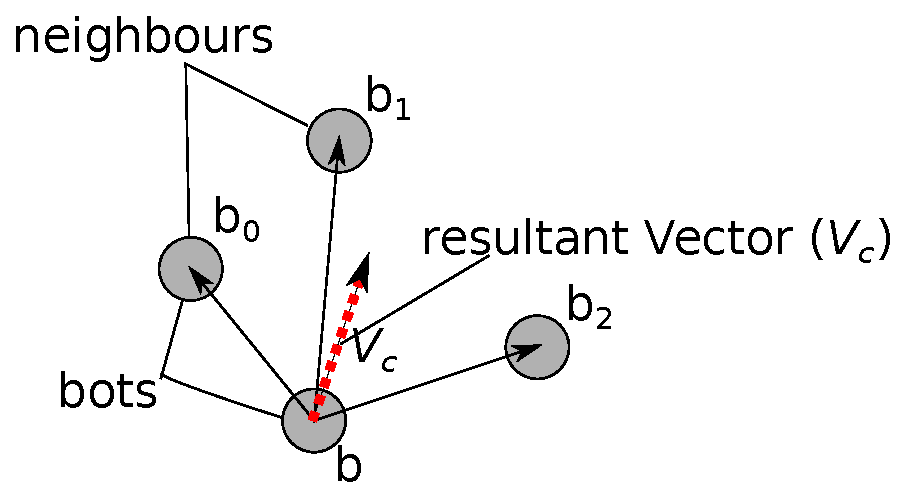
\includegraphics[width=4cm]{figures/FlyToCentre1}
\end{center}
\caption{Cohesion: Origin $b$ \label{methods:FlyToCentre1}}
\end{figure}

The cohesion vector $v_{c}$ for bot $b$ is given by:-
\begin{equation}\label{eq:FlyToCentre1}
v_{c} = \frac{1}{n}{ \sum_{i=0}^{n}} b_i
\end{equation}‎

\subsection{Swarm Repulsion}
Bots in the swarm have a fixed distance/range where by a repulsive vector needs to be applied (\Fig{} \ref{methods:Repulsion1}) as discussed by Miner \cite{MD07}, This creates a field around the bot preventing other bots from moving into a position that could cause a collision. Any bot that moves within the range are directed away by a directional vector equal to the range no mater what the proximity is, the vector is applied in the opposite direction to which the bot approaches by inverting the vector.

\begin{figure}[H]
\begin{center}
\includegraphics[width=4cm]{figures/Repulsion1}
\caption{Bot Repulsion \label{methods:Repulsion1}}
\end{center}
\end{figure}

Where $d_b$ is distance for a given bot and $b_n$ is the vector created between the bot and its neighbour $b_n =‎ \overrightarrow{BB_n}$ ($B$ is the bot and $B_n$ a neighbour) the resultant vector is calculated as:-

\begin{equation}
\label{eq:Repulsion1}
v_{r} =‎ - \sum_{n:|b_n| < d_b^{}} {b_n} \left ( \frac{d_b - |b_n|}{d_b} \right )
\end{equation}‎

For a bot $b$, $v_{r}$ is a repulsive vector generated when a bot approaches to close to another bot. When a bot does move into this area it is repelled in proportion to the amount it has moved into the bot's repulsive area: the proportion is calculated by $\frac{b_{b} - |b_{n}|}{d_b}$. The distance for the repulsive force is $d_b$ which is the distance around the bot where repulsion will be required to prevent a collision. The bots that are within the repulsive area are identified by ${n:|b_{n}| < d_b}$.

\subsection{Swarm Model}

Within a swarm these simple rules of "keep a minimum distance" (repulsion) and "maintain proximity" (cohesion) cause the swarm to form natural geometric structures (hexagons when the repulsive and cohesive fields are correctly set) a feature seen throughout the natural world~\cite{ALMC13}.
If two bots are in close proximity they will naturally adhere to each other due to the proximity rule (\Fig{} \ref{fig:StableForms}). When no other forces act upon bots they will degrade into the most stable system they can in which the bots are equidistant apart with equal angles.
In the case of 3 bots this will be a triangle, in the case of 4 bots this will be a diamond with the centre components joined, with 5 and 6 a triangular lattice will emerge and with 7 bots a stable hexagon will form. The hexagon is the most stable as all structures with all bots being equal distance apart with the same angle.

\begin{figure}[H]
\begin{center}
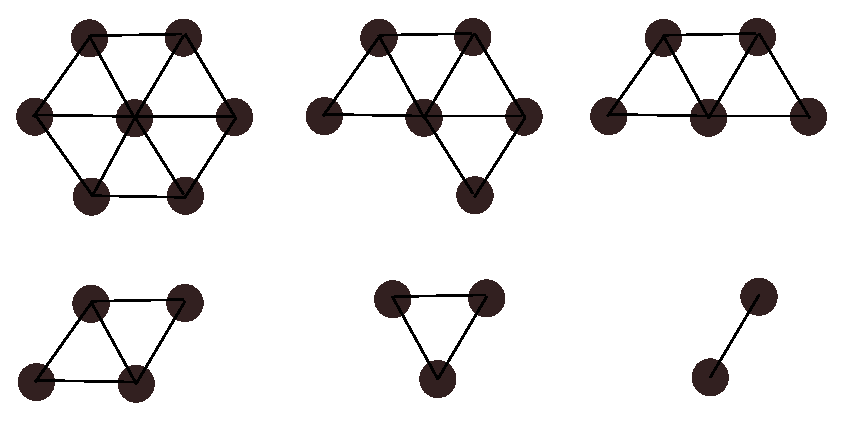
\includegraphics[width=7cm]{figures/StableForms}
\end{center}
\caption{Stable Swarm Formations}\label{fig:StableForms}
\end{figure}

%%======================================================================================================

The directional vector $v$ for bot $b$ (\Fig{} \ref{methods:Repulsion1}) is the normlised sum of the cohesion and repulsion vectors:

\begin{center}
\begin{equation}
\label{eq:BotSwarm1}
v =‎ (v_{c} + v_{r})\string^
\end{equation}‎
\end{center}

\subsection{Swarm Direction}\label{sec:Direction1}
A destination is a point within a Euclidean space for the swarm to migrate towards this gives rise to a destination vector which is added to a bot's cohesion and repulsion. Combining the three vectors creates a final directional vector for the individual bot and in effect for the whole of the swarm. The direction of this vector influences the bot's motion,
not it's magnitude. (\Eq{}~\ref{eq:Destination1})

%%=============================================================================

\begin{figure}[H]
\begin{center}
\includegraphics[width=4cm]{figures/Destination}
\caption{Destination Attraction \label{methods:Destination1}}
\end{center}
\end{figure}

\begin{center}
\begin{equation}\label{eq:Destination1}‎
v_{d} =‎ (BD_0)\string^
\end{equation}‎
\end{center}

\subsection{Bot Direction Calculation}

A bot's direction is a normalised resultant vector of all the forces that act upon it, if we therefore bring together all the force based vectors that have been calculated, a final resultant direction can be derived by summing all the constituent vectors then normalising the result.

\begin{center}
\begin{equation}
\label{eq:BotDirection1}
v =‎ (v_{c} + v_{r} + v_{d})\string^
\end{equation}‎
\end{center}

\subsection{Weighted Model}

\Eq{} \ref{eq:BotDirection1} is limited in terms of how these directional vectors are applied. The model needs to be refined to determine the bot's final directional vector as in \Eq{}~\ref{eq:BotPhysics1}‎. The refinement is achieved by adding a weighting to each of the directional vectors, the weighting simply creates a variation of how much each of the vectors is applied. Each vector is multiplied by its own factor ($k$) that will increase or decrease its effect.

This modelling creates a final directional vector that takes into account all the surrounding influences that effect each bot.

Once the final vector is calculated it must be normalised to a directional vector that will be applied to each bot within the swarm based on the bots speed to give the next cycle of the swarm.

\begin{equation}\label{eq:BotPhysics1}‎
v =‎ (k_cv_c + k_rv_r + k_dv_d)\string^
\end{equation}‎

\subsection{Resultant Bot Model}

The swarm created by the above process will be a 'stable' structure such that the bots will remain connected (\Fig{}~\ref{methods:Stable1}) within the swarm and over time an optimum structure is created as all the resultant forces balance and stabilise.

Most swarms have bots that move, in this paper the bot model is such that the bots move at a constant speed, or if in equilibrium then the resultant null vector (see section \ref{Section:StabilityNullVector}) will mean the bot stops and remain motionless.

\subsection{Swarm Simulations}

Within the simulations used for this paper the swarm is initially created by a random dispersal of the bots (\Fig{}~\ref{methods:Chaos1}). This initial state with the vectors being unbalanced will be referred to as the chaotic state. This chaos is caused by an inequality in the resultant vector magnitudes that are acting upon each of the bots (as detailed above), based upon the application of the weighted model the swarm will initially try to balance all the vectors resulting in the bots moving in what appears to be random directions but the effect is an expansion or contraction of the swarm to its most `stable' state based upon the weighted model constraints.

This phase of the swarm's life cycle can be called the initialisation phase (\Fig{}~\ref{methods:StableTime1}). The vectors that create this `stable' swarm being equal for all the bots (repulsion, cohesion) will result in the most stable shape possible: a hexagonal lattice. This will occur provided the cohesive field is less than twice the repulsive field. The resultant structure will have all the angles and lengths (distances between bots) the same or fluctuating within a small range (\Fig{}~\ref{methods:Stable1}).

This effect can be seen in the simulator snapshots below:-

\begin{figure}[H]
\begin{center}
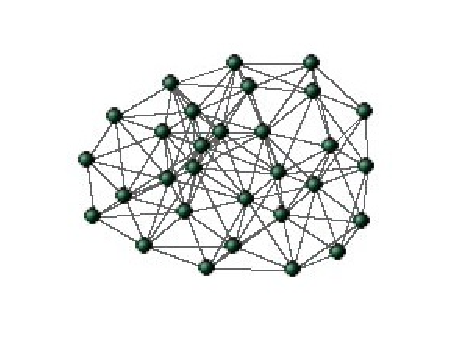
\includegraphics[width=5cm]{figures/Chaos}
\end{center}
\caption{Chaotic Swarm\label{methods:Chaos1}}
\end{figure}
\begin{figure}[H]
\begin{center}
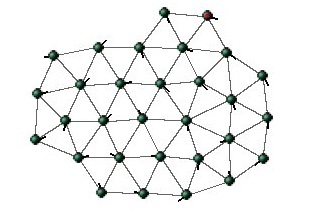
\includegraphics[width=5cm]{figures/Stable}
\end{center}
\caption{Stable Swarm\label{methods:Stable1}}
\end{figure}
\begin{figure}[H]
\begin{center}
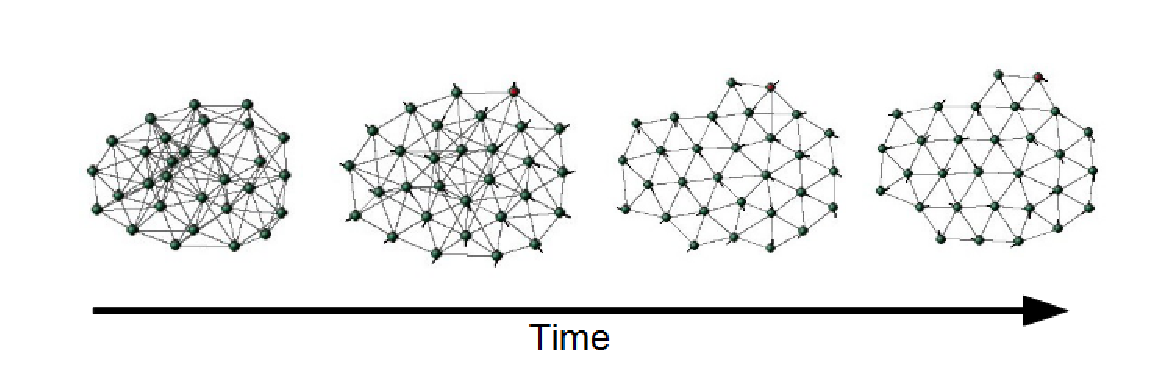
\includegraphics[width=7cm]{figures/StableTime}
\end{center}
\caption{Swarm Stabilisation\label{methods:StableTime1}}
\end{figure}

\section{Swarm Stabilisation\label{section:swarmStabilisation}}
The focus of this paper is the \stability{} of a swarm as it progresses towards a stable form and the variations once it has reached that state.

The swarm under investigation in this paper is a monolithic swarm where the bots within the swarm are identical. The swarm can propagate towards a stable form where the repulsion and cohesion distances are such that the visible distances of the bots are beyond the repulsion range and the repulsion range is more than half of the visible distance. This will ensure that the structure propagates towards a stable hexagonal lattice.

\section{Swarm Dynamic Metrics\label{methods:SwarmStability}}
The paper will now look at two ways of measuring \stability{} in a swarm.

One method is through the balancing of the cohesive and repulsive magnitudes that exist between the bots in a swarm \cite{VGKP11} \cite{LBMFKV07}. The more the overall magnitude tends towards zero for a swarm then the less \stability{} there is within the swarm; however at any point in time there may be an imbalance between the repulsive and the attractive forces therefore the deviation from the mean also needs to be considered.

The other metric that will be considered is the constancy in the inter bot distances. At any point in time the distances between the bots, in a neutral swarm, should tending towards all being equal resulting in no movement. Again the variation is important to determine the \stability{} therefore it is important to consider the standard deviation from the average as an additional measure of \stability{}. If the standard deviation is zero then all the bots are evenly spaced.

\subsection{Magnitude Dynamics}

Magnitude based \stability{} is measured by the balance between the repulsion and adhesion between the bots with a swarm. In this model there is an area around a bot where repulsion will come into play (\Fig{}~\ref{methods:FlyToCentre1}, \Eq{}~\ref{eq:Repulsion1}).
Here the repulsion increases progressively as the bots' positions converge. At the same time as the repulsive vector is being calculated and applied the cohesive vector is being calculated based on neighbour proximity and causing the bots to move towards each other (\Fig{}~\ref{methods:Repulsion1}, \Eq{}~\ref{eq:FlyToCentre1}).

At the point at which these two forces balance (equilibrium) there will be no directional bias. This will cause the bots to move in a manner such that there will be no variation in the distances between each other. However given the nature of the bots movements, a constant speed, it his highly unlikely that this perfect balance will be obtained. The resultant motion can be considered as the minimum \stability{} that can be obtained in so much as there will be no or limited variation in how far apart the bots are varying (jitter) and the structure of the swarm will be predictable. Due to the dynamic nature of a swarm, however, maintaining complete \stability{} as in (\Fig{}~\ref{methods:Stability4}, \Eq{}~\ref{eq:Stability4}) is highly unlikely and all the bot pairs will fluctuate between the 3 states of (\Figs{} \ref{methods:Stability2}, \ref{methods:Stability3}, \ref{methods:Stability4}, \Eqs{}~\ref{eq:Stability2}, \ref{eq:Stability3}, \ref{eq:Stability4}).
This transition between the three states is jitter. The degree of jitter is determined by the deviation in the resultant magnitude of the vectors created by the bots displacements within the swarm as a whole.

\begin{figure}[H]
\begin{center}
\includegraphics[width=6cm]{figures/Stability1}
\end{center}
\caption{\Stability{} cohesion (no repulsion)} \label{methods:Stability1}
\end{figure}

\Fig{} \ref{methods:Stability1} shows two bots within each others `visible' feilds but not close enough for repulsion.
In this case $k_cv_c > 0$ and $k_rv_r = 0$.

\begin{figure}[H]
\begin{center}
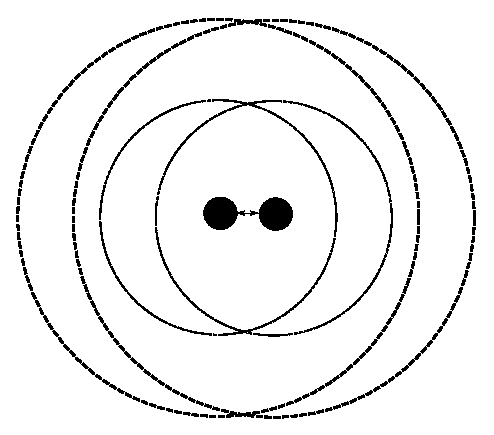
\includegraphics[width=4cm]{figures/Stability2}
\end{center}
\caption{\Stability{} Repulsion} \label{methods:Stability2}
\end{figure}

\Fig{} \ref{methods:Stability2} shows two bots close together with repulsion dominating cohesion: $k_cv_c < k_rv_c$. The resultant vector will direct the bots away from each other.

\begin{figure}[H]
\begin{center}
\includegraphics[width=4cm]{figures/Stability3}
\end{center}
\caption{\Stability{} cohesion} \label{methods:Stability3}
\end{figure}

\Fig{} \ref{methods:Stability3} shows two bots close together but with cohesion dominating: $k_cv_c > k_cv_c$. The resultant vector will draw the bots together.

\begin{figure}[H]
\begin{center}
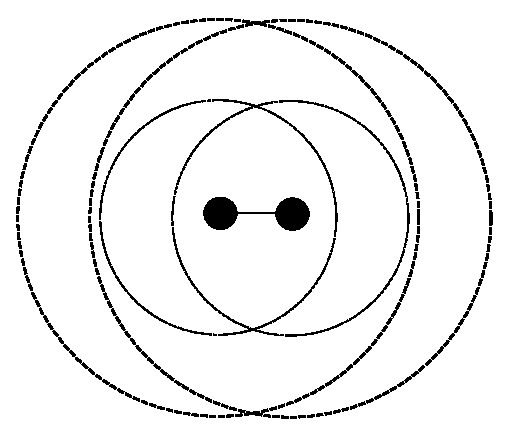
\includegraphics[width=4cm]{figures/Stability4}
\end{center}
\caption{\Stability{} equilibrium} \label{methods:Stability4}
\end{figure}

\Fig{} \ref{methods:Stability4} shows two bots close together with $k_cv_c == k_rv_r$ the resultant vector will be a \textit{null vector} and the bots will have no effect on each other.

\subsubsection{\Stability{} using magnitude}\label{Section:StabilityMagnatude}

The model so far is using both vectors (cohesion, repulsion) and the resultant vector magnitudes as a means to identify the directional influence the swarm incorporates in its movement. These are not new concepts in terms of measuring stability. The use of the magnitudes comes from the fact that when looking at the swarm in terms of each bot's relationship with its neighbours we are in fact looking at two bots at a time. The effect of this is that for each directional calculation the cohesion and repulsion vectors are on the same line (\Fig{}~\ref{methods:Stability5}). This results in the vectors magnitudes being a means of identifying the amount of influence that is resultant for the bot pair.

by $k_cv_c < k_rv_r$ we mean the magnitudes of the vectors which are aligned along the line of separation between the bots.

\begin{figure}[H]
\begin{center}
\includegraphics[width=4cm]{figures/Stability5}
\end{center}
\caption{Vectors on line of separation} \label{methods:Stability5}
\end{figure}

\subsubsection{\Stability{} and the null vector}\label{Section:StabilityNullVector}

Having no \Stability{} is in effect an attempt of the system to create a situation where by all the vectors of cohesion and repulsion cancel out such that the resultant directional vector is a null vector.

If we consider the equilibrium state (\Fig{}~\ref{methods:Stability4}) the resultant vector will be $r = (0,0)$. note: you cannot normalise a null vector! (division by zero error) ($\hat{v} = \frac{v}{|v|}$ if $v\neq0$; $0$ if $v=0$) If the resultant vector $r$ is normalised $|r|$ then the resultant vector is $(0,0)$ a null vector. The resultant vector $r$ is used to determine movement that is to be applied at the next time interval $t$. The effect of a null vector is that the bot will remain stationary~(\Fig{}~\ref{methods:StabilityNullVector}).

\begin{figure}[H]
\begin{center}
\includegraphics[width=6cm]{figures/StabilityNullVector}
\end{center}
\caption{Equilibrium with null vectors} \label{methods:StabilityNullVector}
\end{figure}

Due to the movements within the swarm as a whole this situation is very rare as each bot interacts with its neighbours. This residual motion is the background `noise' that an algorithm creates.

If the swarm has no other external factors acting upon it and all the bots achieve the ideal distances and angles then there will be no motion (\Fig{} \ref{methods:StabilityNullVector}). If there are any other factors, then there may motion such as a directional goal based swarm, it is however very unlikely that a completely motionless situation will arise.~(\Fig{}~\ref{methods:StabilityNullVector2})

\begin{figure}[H]
\begin{center}
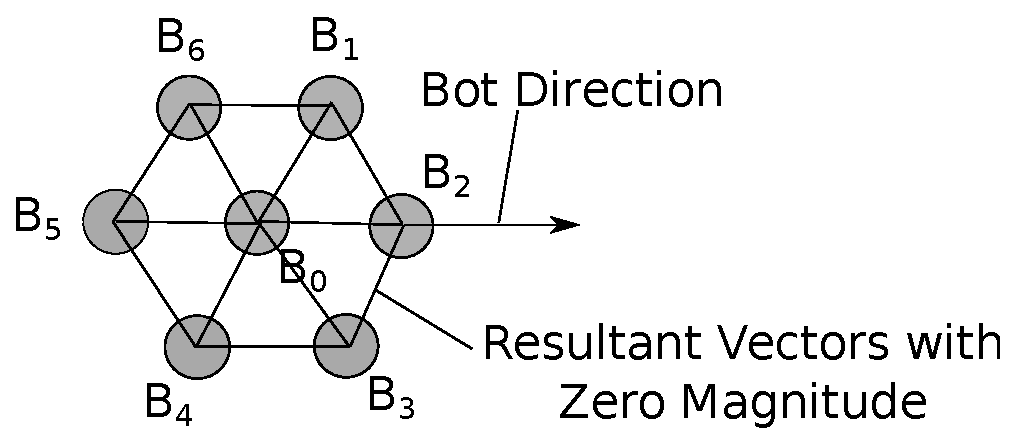
\includegraphics[width=6cm]{figures/StabilityNullVector3}
\end{center}
\caption{Directional movement and null vector (t)} \label{methods:StabilityNullVector3}
\end{figure}

\begin{figure}[H]
\begin{center}
\includegraphics[width=6cm]{figures/StabilityNullVector2}
\end{center}
\caption{Directional Movement and null vector (t + 1)} \label{methods:StabilityNullVector2}
\end{figure}

\subsubsection{Magnitude based \Stability{} Model}\label{Section:StabilityModel}

With the definition of the magnitude based \stability{} given it is now possible to apply the model to the whole of the swarm. If we now take every bot it is possible to calculate a resultant magnitude created between itself and its neighbours. Taking each neighbour a resultant magnitude can be calculated by subtracting the effective cohesion and repulsion generated between the two bots. Taking the absolute value for that pair and all the other neighbours give a resultant distance that can be used as a metric to identify the \stability{} of the specific bot in terms of its position in the swarm.

Using the formulae for the calculation of both cohesion ($C$) (\Eq{}~\ref{eq:FlyToCentre1}) and repulsion ($R$) (\Eq{}~\ref{eq:Repulsion1}) for every bot and its neighbours it is also possible to calculate an overall value (sum of magnitude) that can represent the overall stability of the swarm. The closer the metric is to zero the more 'stable' the swarm.


\begin{equation}
\label{eq:BotStabilityT}
D(b,t) = \sum_{i=1}^{n}(||C(b(t),b_{i})|| - ||R(b(t),b_{i})||)
\end{equation}

$D(b,t)$ is the overall magnitude for bot $b$ and $b_i$ are the neighbours of $b$ and $t$ is the point in time of the simulation. The internal metric is the average over the swarm:

%\begin{equation}
%\label{eq:SwarmStability}
%S = \sum_{j=1}^{n}D(b_j)
%\end{equation}

%Where $S$ is the stability metric and $D$ takes as a parameter each bot $b_j$ which is for the
%whole swarm and returns the overall magnitude for swarm.

%This metric can be used to compare swarm stability by producing an average stability per bot
%(Formulae. \ref{eq:SwarmStabilityQuotient}) for a given
%algorithm or swarm.

\begin{equation}
\label{eq:SwarmStabilityMetricT}
\mu(t) = \frac{1}{n}{\sum_{j=1}^{n}D(b_j,t)}
\end{equation}

This provides a means of comparing swarms of any size or utilising any control algorithm and $t$ is the point in time the reading is taken.

\subsubsection{Variance in \stability{}}\label{Section:VarienceInStability}

The mechanism above provides an overall indication of the \stability{} based on inter bot vectors. This model however gives an indication of \stability{} as an overall metric. To improve the analysis a further clarification is required in terms of the variation from the \stability{} metric. Calculation of the \stability{} metric is the standard deviation of the entire swarm from the norm (mean) of the inter bot forces.

The mean of the forces is calculated as swarm \stability{} metric above
(\Eq{}~\ref{eq:SwarmStabilityMetricT}).

The standard deviation is calculated as:-

\begin{equation}
\label{eq:SwarmStabilityQuotientT}
\sigma(t) = \sqrt{\frac{\sum_{j=1}^{n}(D(b_j,t)-\mu(t))^2}{n}}
\end{equation}

The true metric therefore for the overall \stability{} is the mean and the standard deviation of the swarms internal resultant magnitudes derived from each bots vectors effected by its neighbours.

\subsection{Distance based \Stability{}}

Distance based \stability{} is achieved when there is a balance between the cohesion and repulsion between the bots within a swarm such that it generates an even latice/network of bots. The network can be of any `stable' network type such as a hexagonal latice or a regular graph structure (\ref{methods:SwarmTypesStability1}).

When this state is met the swarm can be analysed in terms of the resultant distances and the variations within that specific state.

\subsubsection{Calculating distance based \stability{}}

The vector generated for a bot $b$ to its neighbour $b_i$, $bb_i$, is as shown in (\Eq{}~\ref{eq:FlyToCentre1}). The magnitude of that vector gives the distance apart of the two bots.

To calculate the average distance for the bots:-

\begin{equation}
\label{eq:SwarmStabilityDistance1}
\mu(t) = \frac{1}{m}{\sum_{k=1}^{m}}\frac{1}{k}{\sum_{j=1}^{n}||b_k(t)b_j||}
\end{equation}

Where $j$ ranges over the neighbours, $k$ ranges over the bots in the swarm.

The deviation from the norm is calculated by:-

\begin{equation}
\label{eq:SwarmStabilityQuotientT}
\sigma(t) = \sqrt{\frac{\sum_{k=1}^{m}\sum_{j=1}^{n}((||b_k(t)b_j||)-\mu(t))^2}{mn}}
\end{equation}

The distance metric therefore for the overall \stability{} is the mean and the standard deviation of the swarms internal resultant distances from each bot, which is created by the repulsion and cohesion vectors that are applied to each bot and its neighbours.

\section{\swarmA{} and \swarmB{} swarms\label{methods:SwarmTypesStability1}}

Based upon changing of the repulsion and cohesion fields as described in (\Fig{}~\ref{methods:SwarmStability}) it is possible to create swarms with different characteristics. If the goal of the swarm algorithm is to produce as swarm that maximises the coverage of the bots by making maximum use of the swarms capability to distribute itself over an area as a hexagonal latice then the cohesion feilds of each bot should not be allowed to propagate beyond a neighbour to the extent that it allows another bot to be identified, this will produce a \textit{\swarmA{}} swarm. If the visibility does extend beyond to the point that there is visibility beyond a neighbour then there will be additional vectors considered in the swarm structure and its properties will change in such a way that the even latice structure will breakdown and create a \textit{\swarmB{}} swarm.

\subsection{\Stability{} testing}\label{Section:StabilityTesting}

During all the testing the model is based upon an interval rate of 100ms.

\begin{center}
\begin{table}[H]
\begin{tabular}{ c | c | c | p{3cm}}
\bf Weight \\\bf Component & \bf \swarmA{} & \bf \swarmB{} & \bf Description \\ \hline
Sample Rate & 100 & 100 & ms - Unit sampling interval\\  \hline
$k_c$ & 5 & 5 & weight adjuster for cohesion bias\\  \hline
$k_r$ & 15 & 15 & weight adjuster for repulsion  bias\\  \hline
$k_d$ & 0 & 0 & weight adjuster for directional bias\\  \hline
Neighbour \\ Distance & 50 & 60 &  units\\  \hline
Bot \\ Boundary & 40 & 40 & units\\  \hline
Speed & 20 & 20 & units/interval\\  \hline
\end{tabular}
\caption{Swarm Weighted Model} \label{tab:Physics2}
\end{table}
\end{center}

The selected options above for the neighbour distance and the repulsion feilds will create the two types of swarm of interest, the distances combined with the weightings are all that is required.

When these two swarm types are simulated from the same base swarm distribution the two swarm types' \stability{} can be analysed.

%%==============================================================================================================

\subsection{\swarmA{} swarm analysis}

Using the formulae created above the two swarm types can be analysed. The magnitude and distance analysis graphs for a \swarmA{} swarm show the initial chaotic swarm settling over the initial 50 * 100ms. The swarm then enters a phase where the hexagons have formed and the average distances between the bots fall and then settle to a more calm phase where the swarm movement is purely the internal agitation required to maintain its structure.

\begin{figure}[H]
\begin{center}
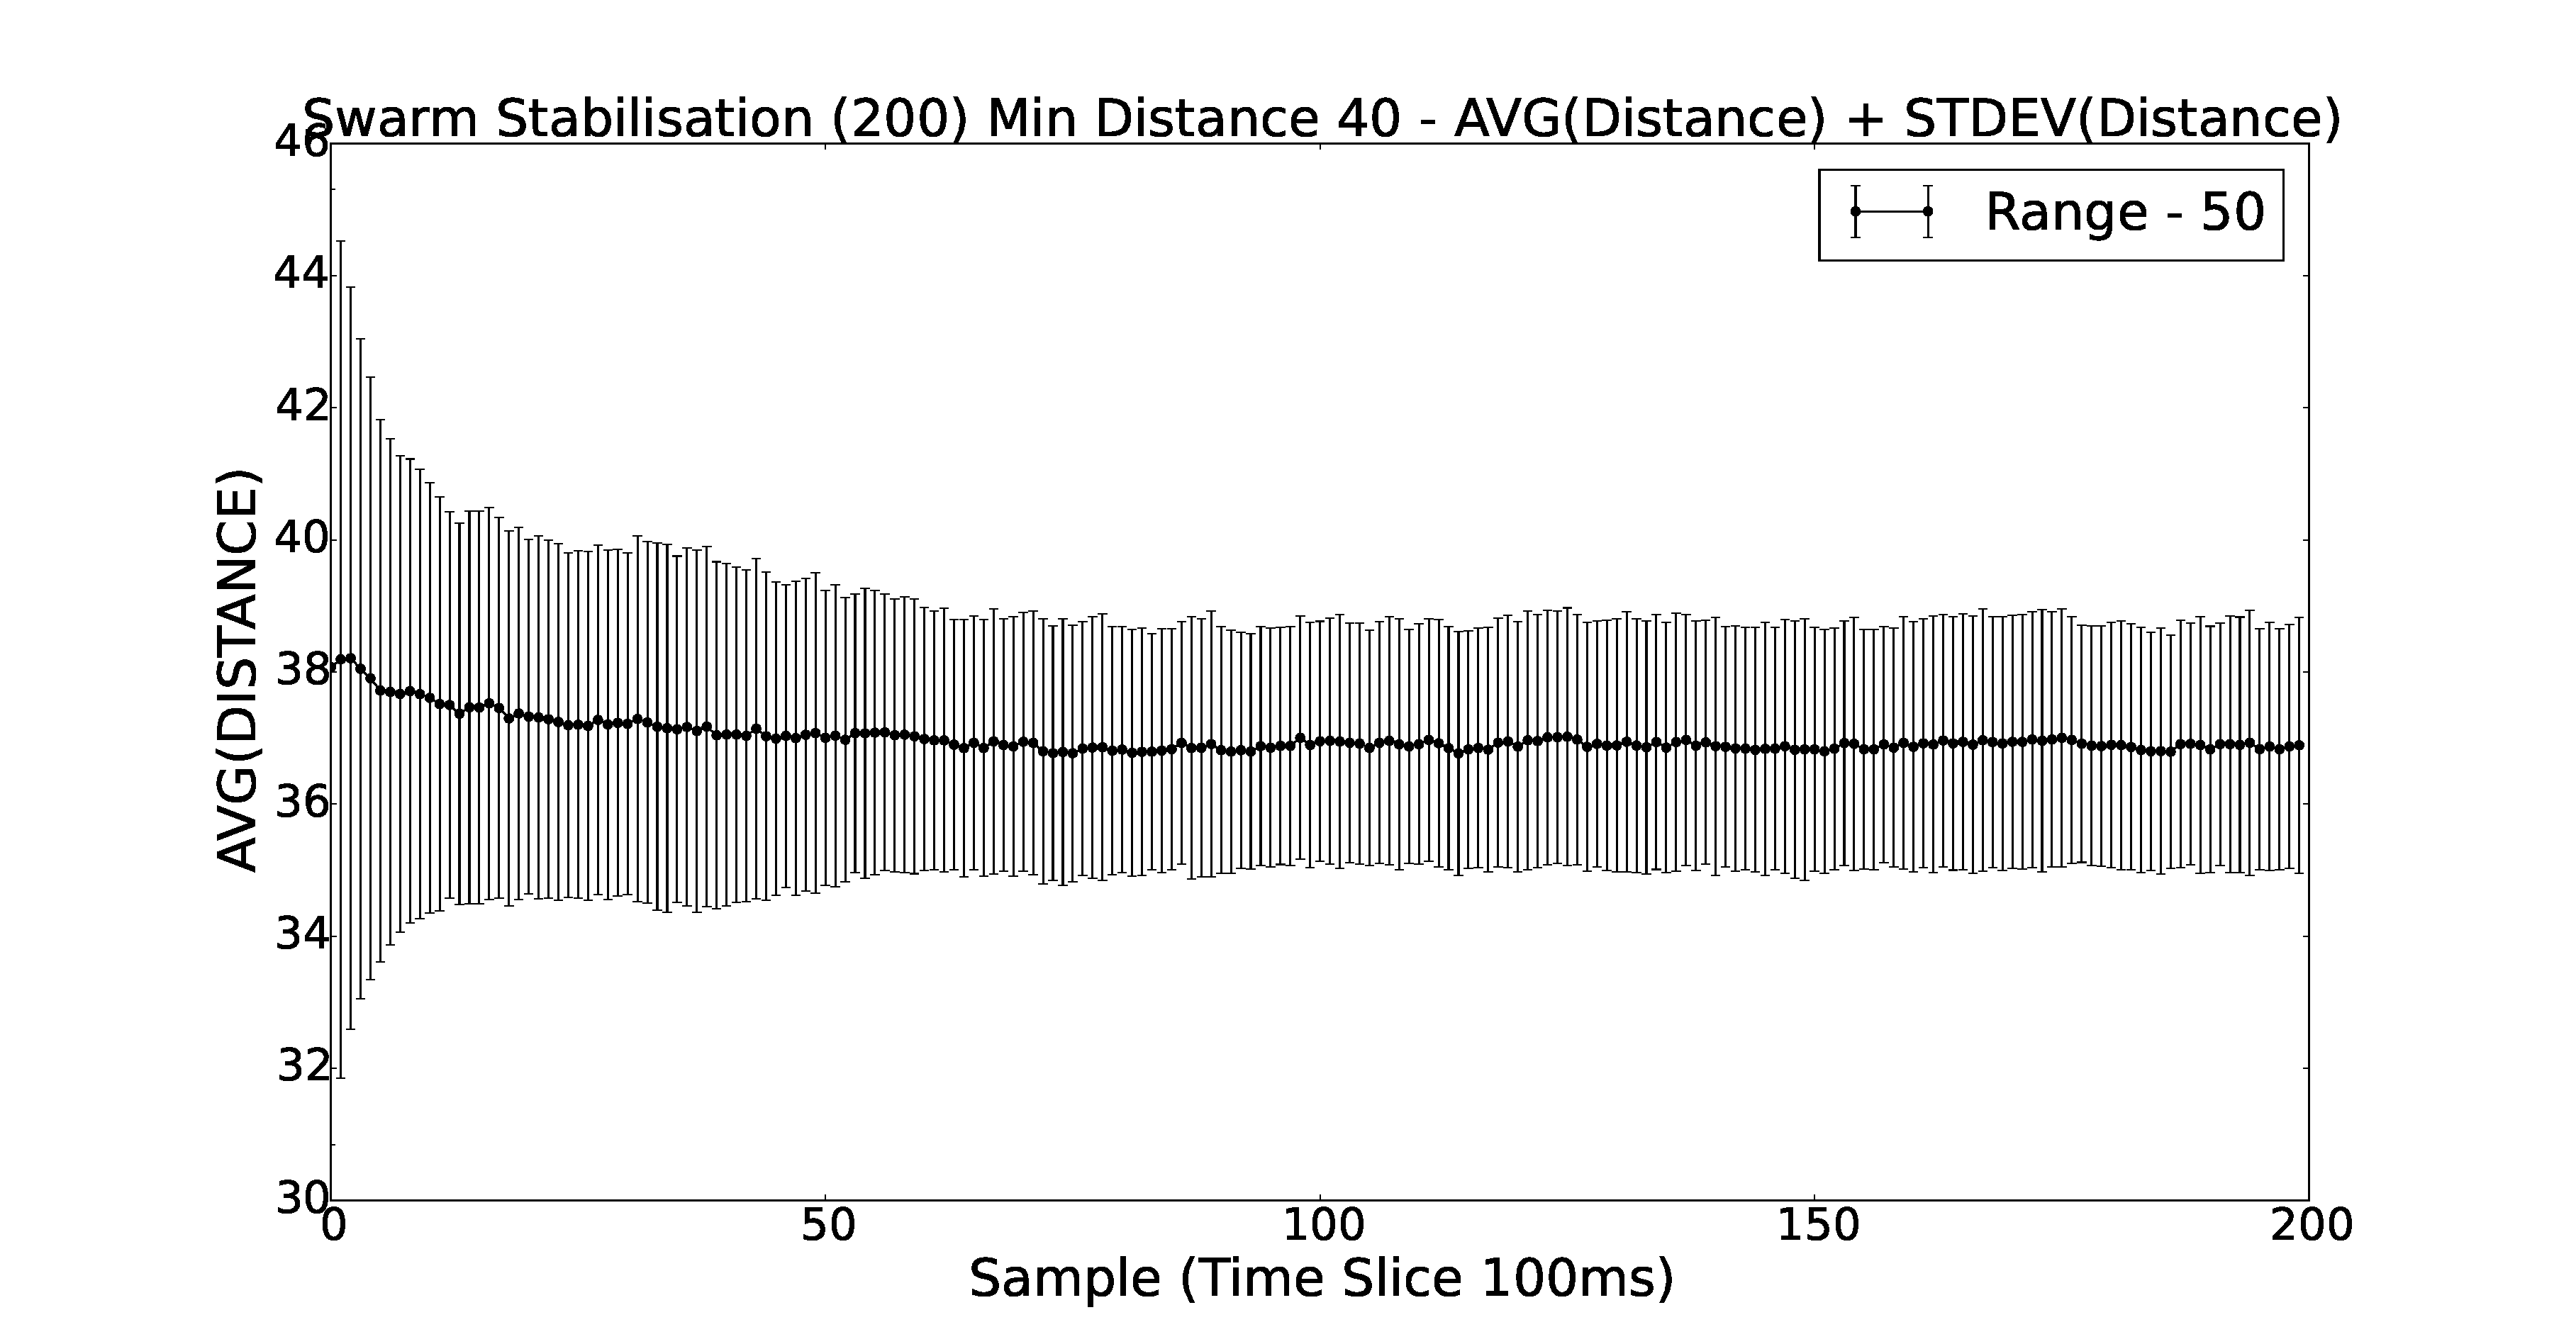
\includegraphics[width=9cm]{figures/StabilityDistanceSwarm40-50}
\end{center}
\caption{Distance stability\label{methods:StabilityDistanceSwarm40-50}}
\end{figure}

\begin{figure}[H]
\begin{center}
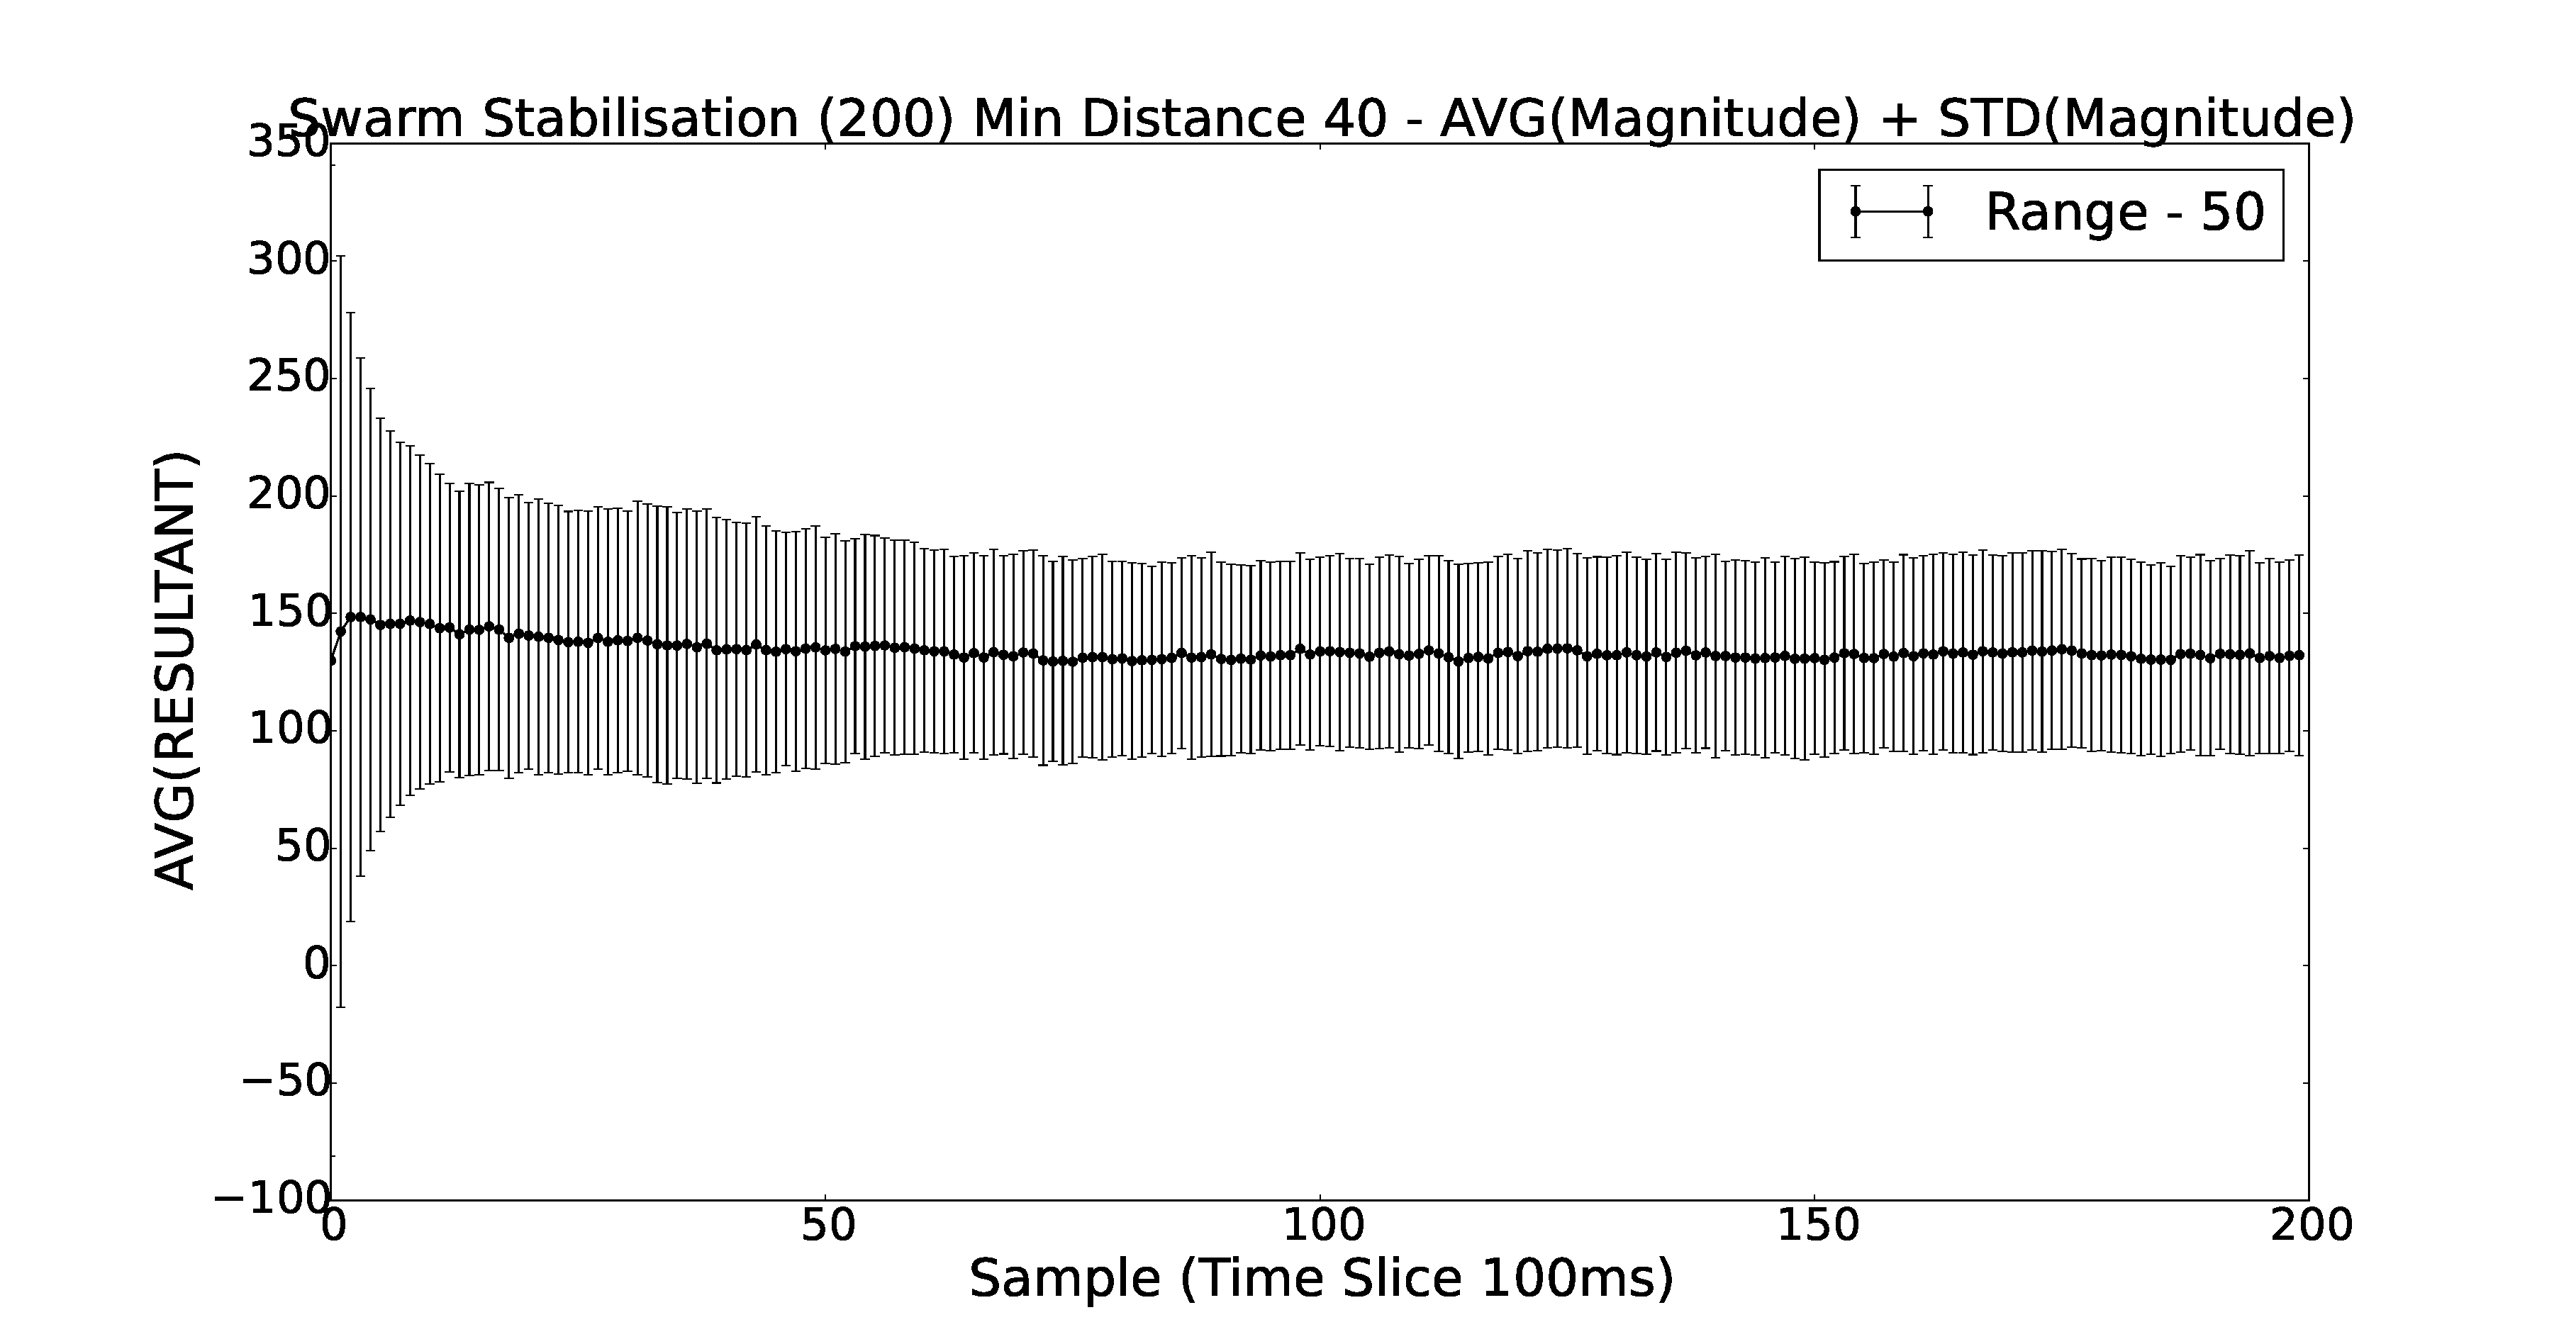
\includegraphics[width=9cm]{figures/StabilityMagnitudeSwarm40-50}
\end{center}
\caption{Magnitude based \stability{}\label{methods:StabilityMagnitudeSwarm40-50}}
\end{figure}

\subsection{\swarmB{} swarm analysis}

\begin{figure}[H]
\begin{center}
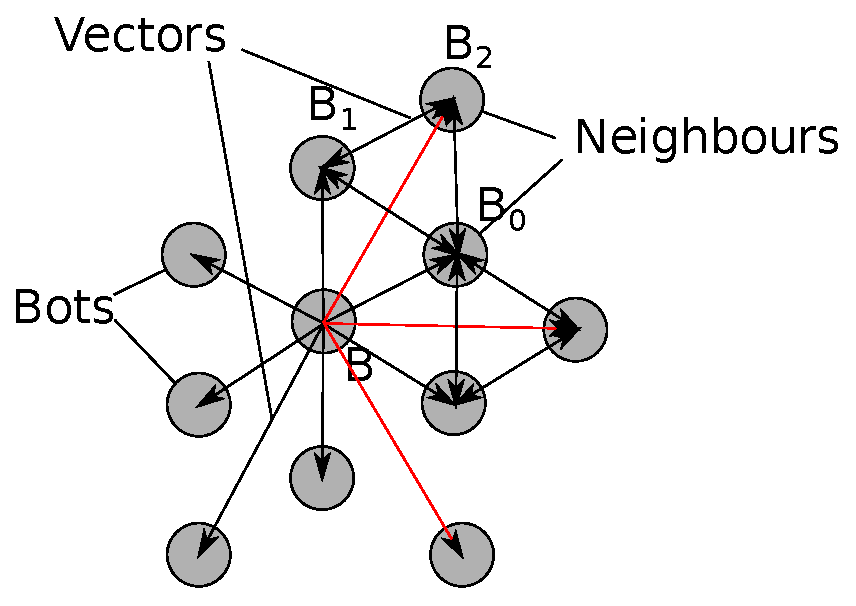
\includegraphics[width=6cm]{figures/CrushedStability}
\end{center}
\caption{\Stability{} in a \swarmB{} swarm} \label{methods:CrushedStability1}
\end{figure}

\begin{figure}[H]
\begin{center}
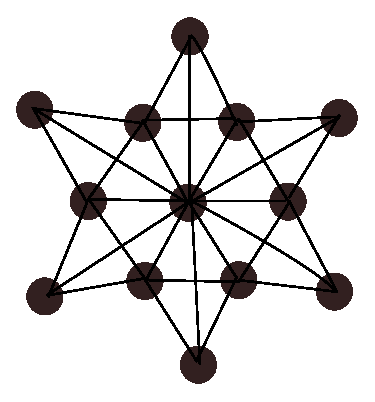
\includegraphics[width=4cm]{figures/StableFormsCompressed}
\end{center}
\caption{\swarmB{} structure} \label{methods:StableSwarmCompressed}
\end{figure}

When the swarm parameters create a \swarmB{} swarm the inter connectivity of the bots is uniform but not hexagonal (\Fig{}~\ref{methods:CrushedStability1}), it is detectable in terms of how the \stability{} metrics present themselves. When a swarm exhibits this type of \stability{} (\swarmB{}) the resultant magnitudes cause the swarm to become very inflexible and so appears 'stable' in terms how overall structure is maintained (\Fig{}~\ref{methods:StableSwarmCompressed}), however there is a great variation in the resultant magnitudes and resultant distances therefore although the distances will maintain a good sound structure the deviations from the average overall swarms magnitudes is visible as high standard deviation within the swarm.
This elevated standard deviation (\Figs{}~\ref{methods:StabilityDistanceSwarm40-60},~\ref{methods:StabilityMagnitudeSwarm40-60}) indicates clearly that the swarm is not at its optimum as the swarm could be distributed further to cover a greater area without effecting the cohesive property.

\begin{figure}[H]
\begin{center}
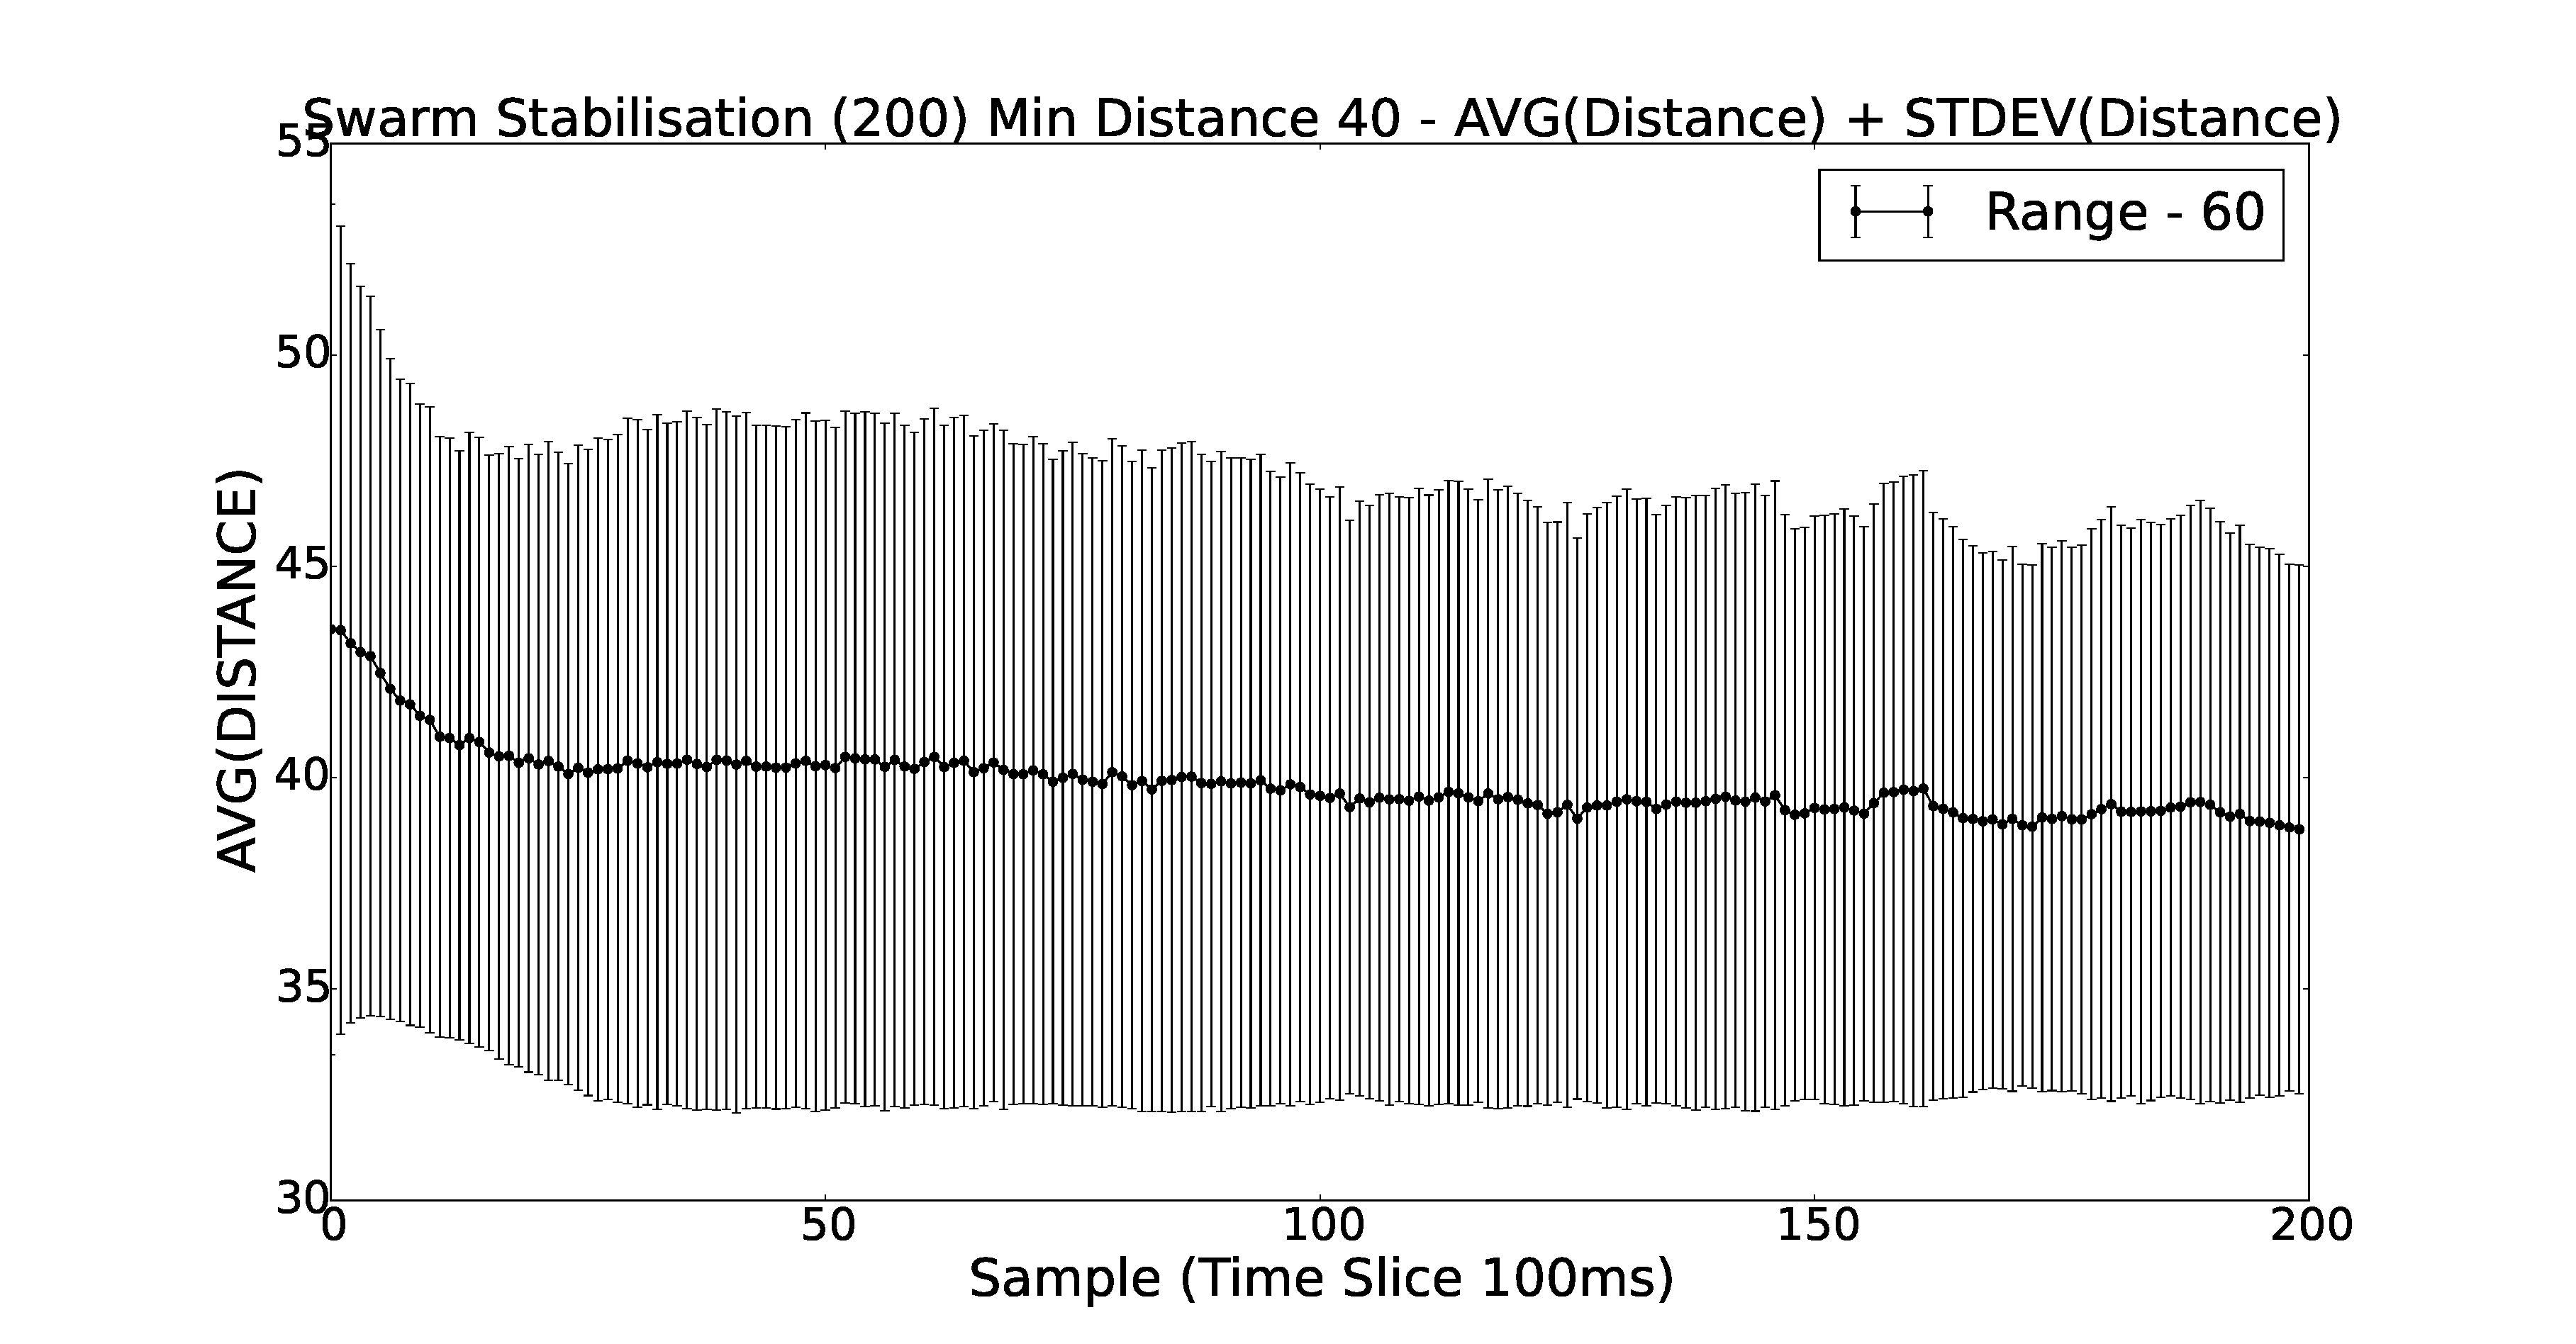
\includegraphics[width=9cm]{figures/StabilityDistanceSwarm40-60}
\end{center}
\caption{Distance based \stability{} \swarmB{}\label{methods:StabilityDistanceSwarm40-60}}
\end{figure}

\begin{figure}[H]
\begin{center}
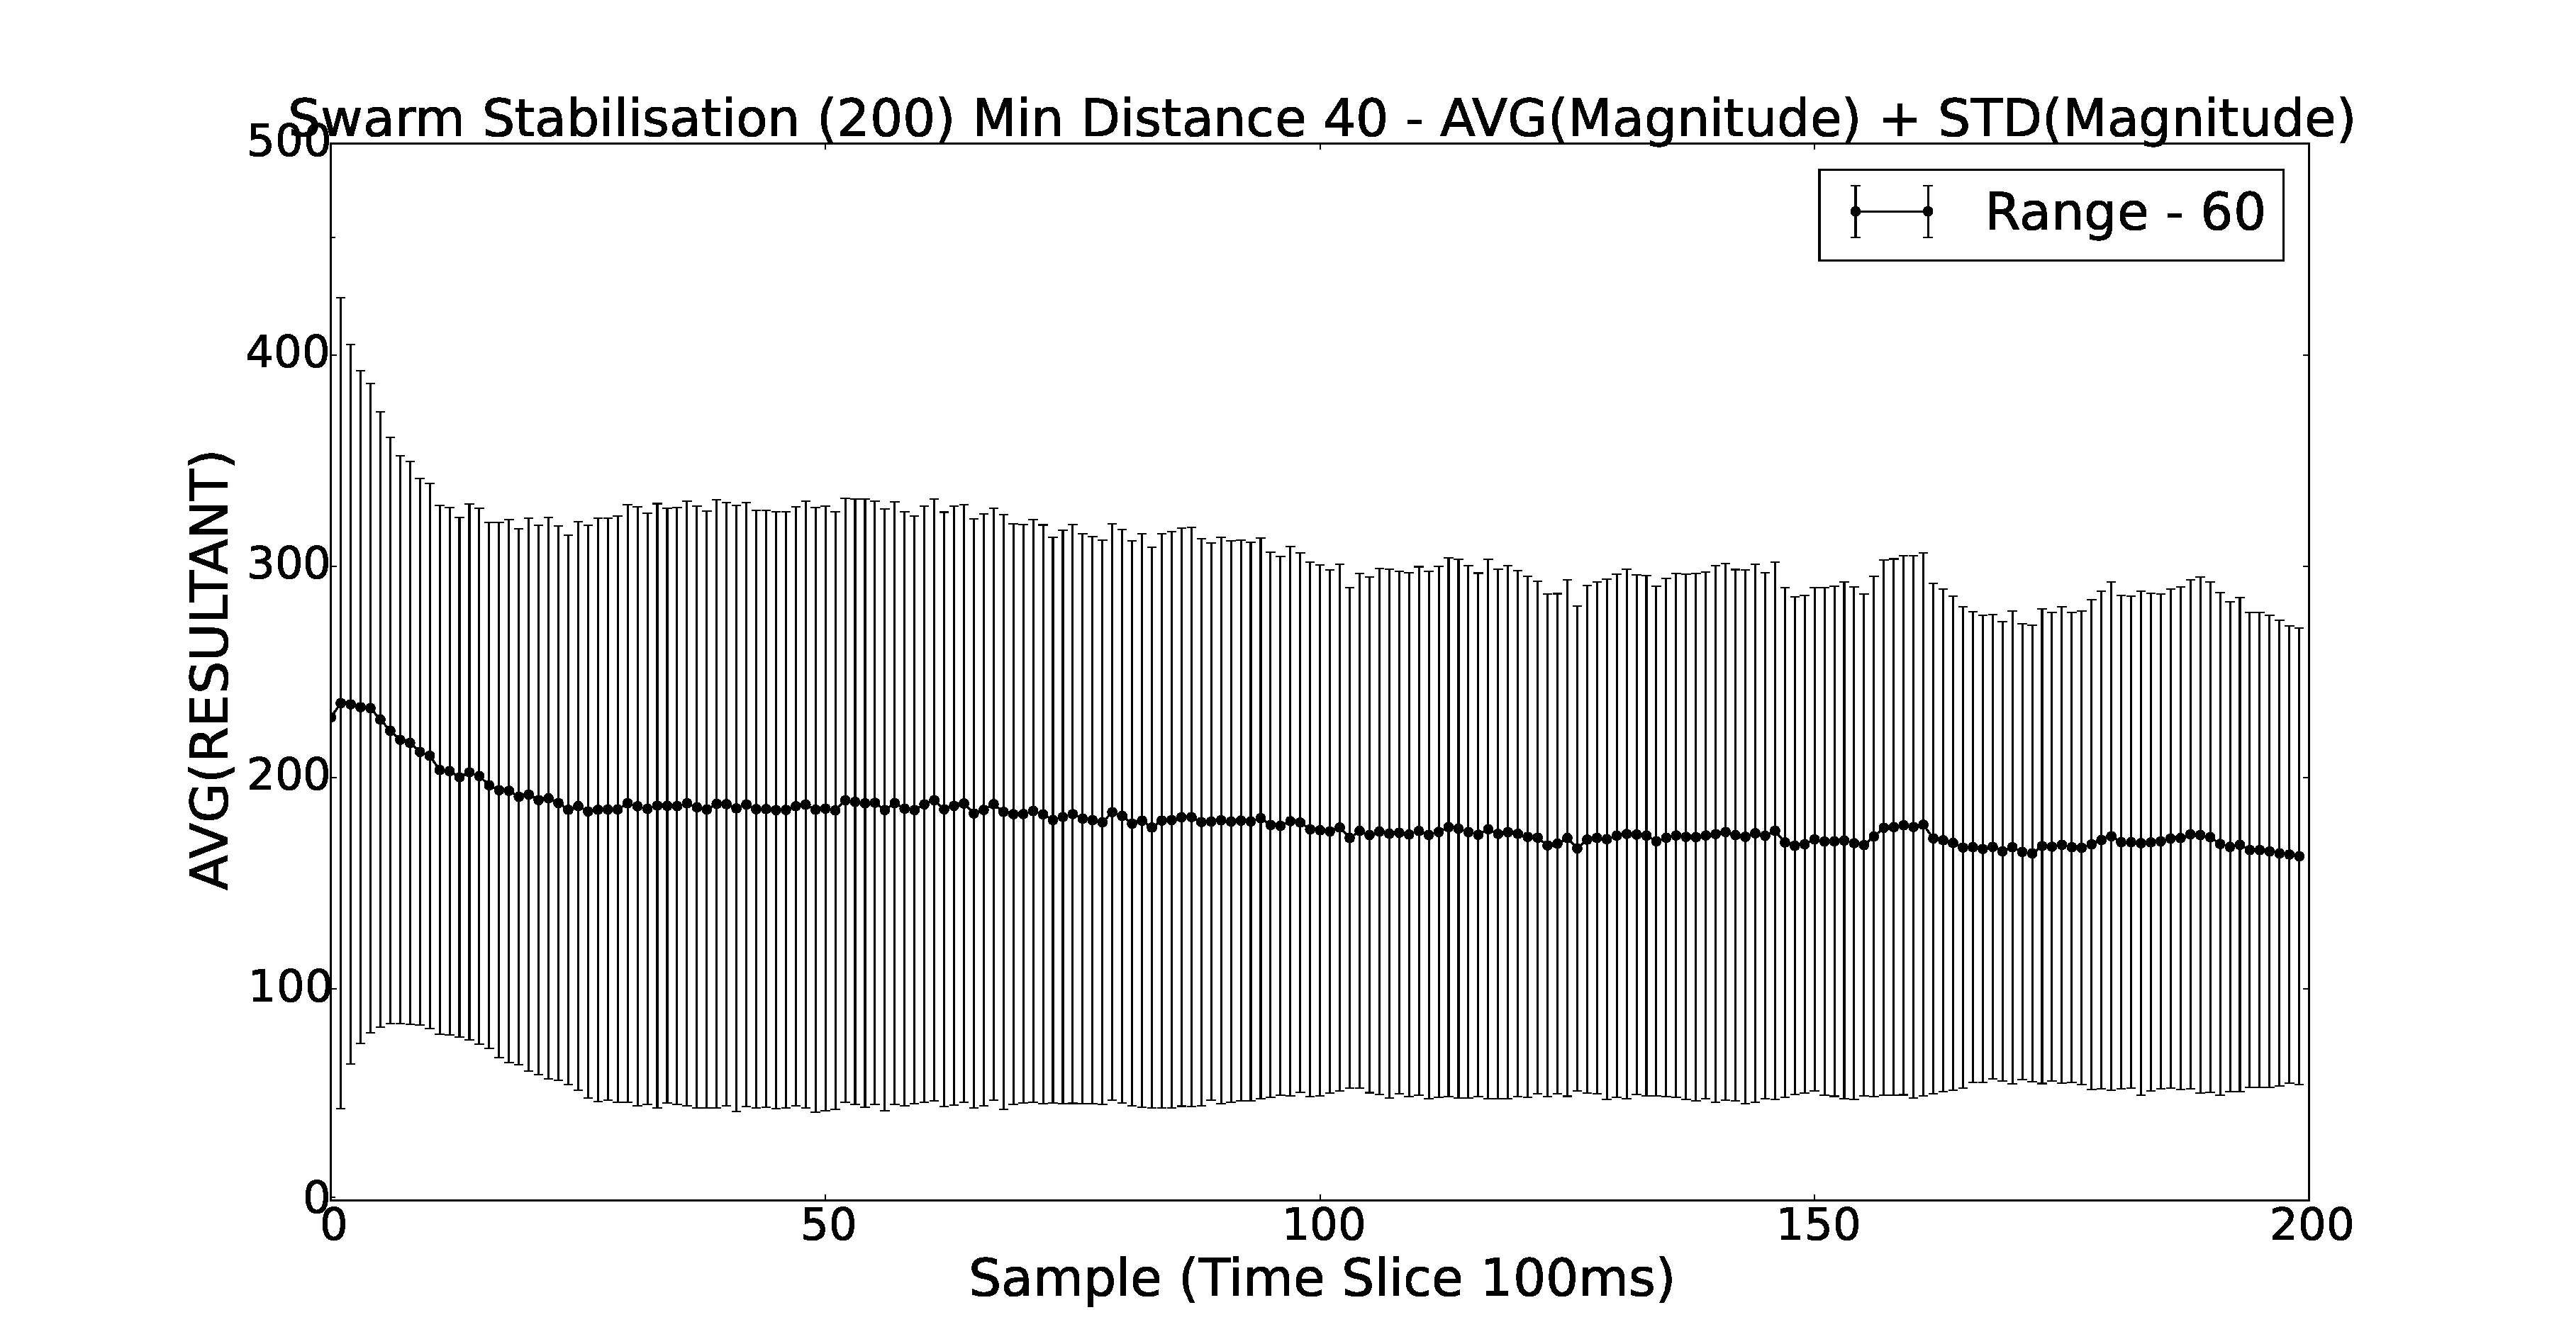
\includegraphics[width=9cm]{figures/StabilityMagnitudeSwarm40-60}
\end{center}
\caption{Magnitude based \stability{} \swarmB{}\label{methods:StabilityMagnitudeSwarm40-60}}
\end{figure}

\section{\Stability{} comparison \swarmA{}/\swarmB{}\label{section:stabilityComparison}}

If we therefore look at the two swarm types together it is evident that the characteristics of the swarm types present themselves as change in the standard deviation from either the average distance or the average magnitude of the bots in the swarm.

The graph (\Fig{} \ref{methods:StabilityDistanceSwarm40-5060}) shows the same swarm with two different field effects for cohesion. The metric used in this analysis is based upon the distances between the bots. The result show that the deviation on the highly connected mesh (shown in black) has a higher standard deviation as opposed to the more hexagonally connect swarm (shown in red).

The graph (\Fig{} \ref{methods:StabilityMagnitudeSwarm40-5060}) shows the exact same swarms as above but in this case the analysis is of the resultant magnitude between the bots in the swarm.

\begin{figure}[H]
\begin{center}
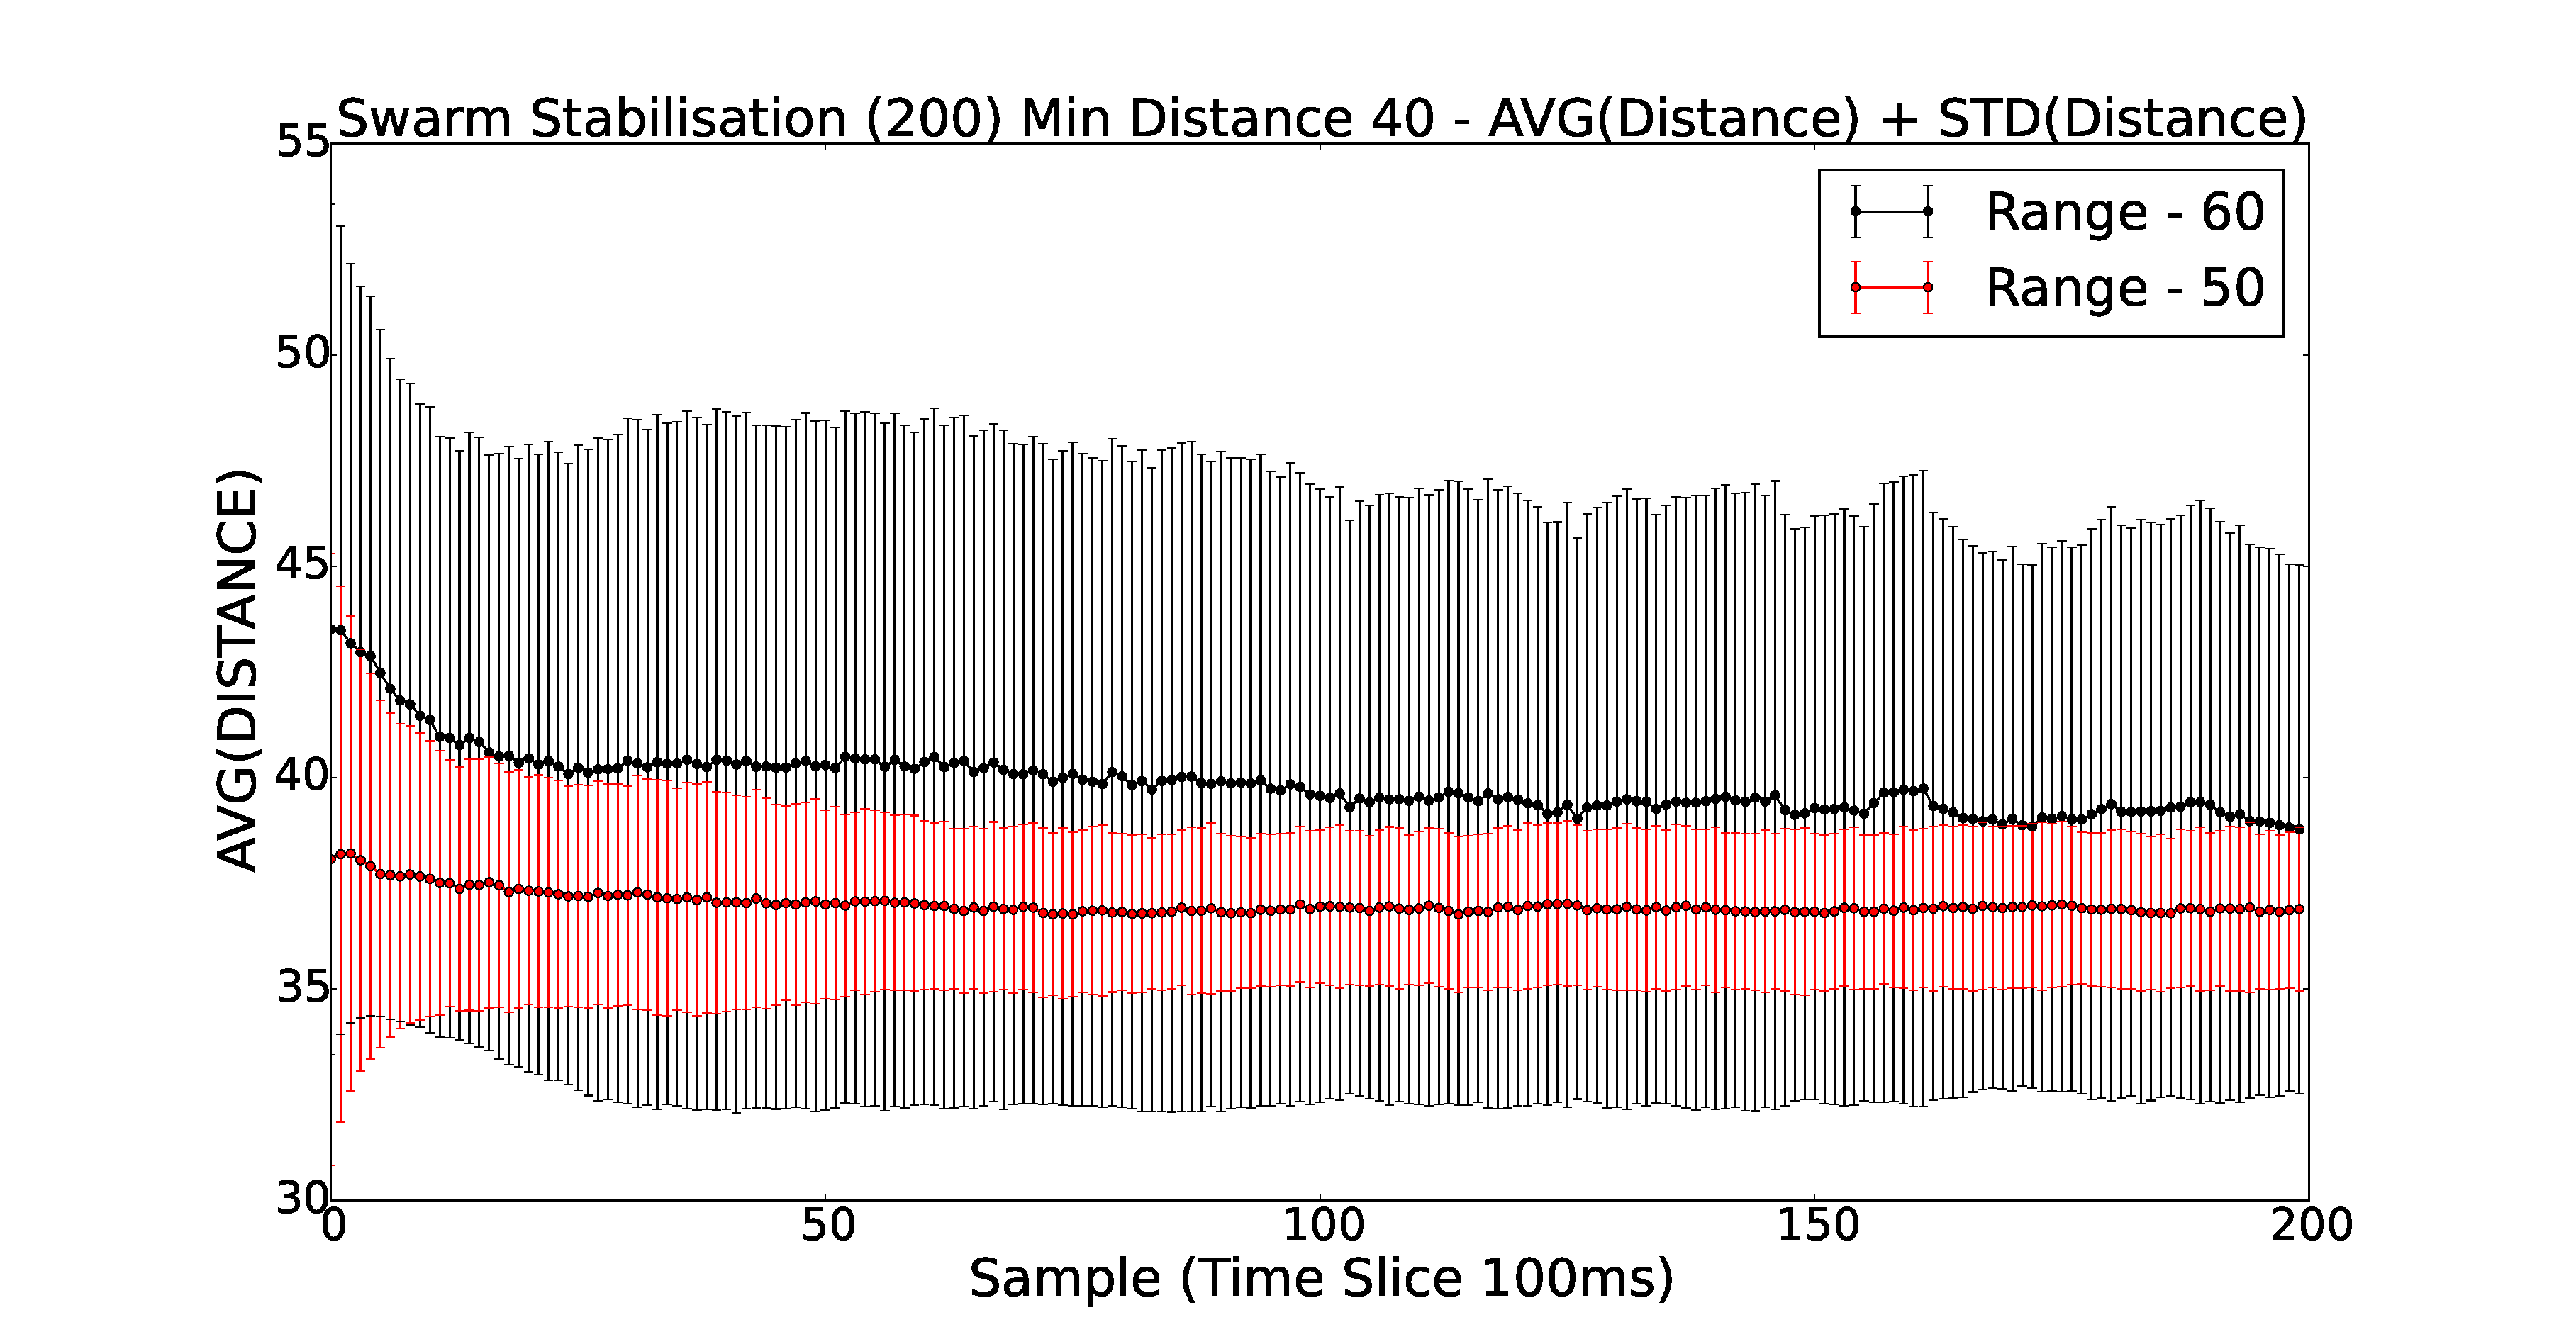
\includegraphics[width=9cm]{figures/StabilityDistanceSwarm40-5060}
\end{center}
\caption{Distances based \stability{}\label{methods:StabilityDistanceSwarm40-5060}}
\end{figure}

\begin{figure}[H]
\begin{center}
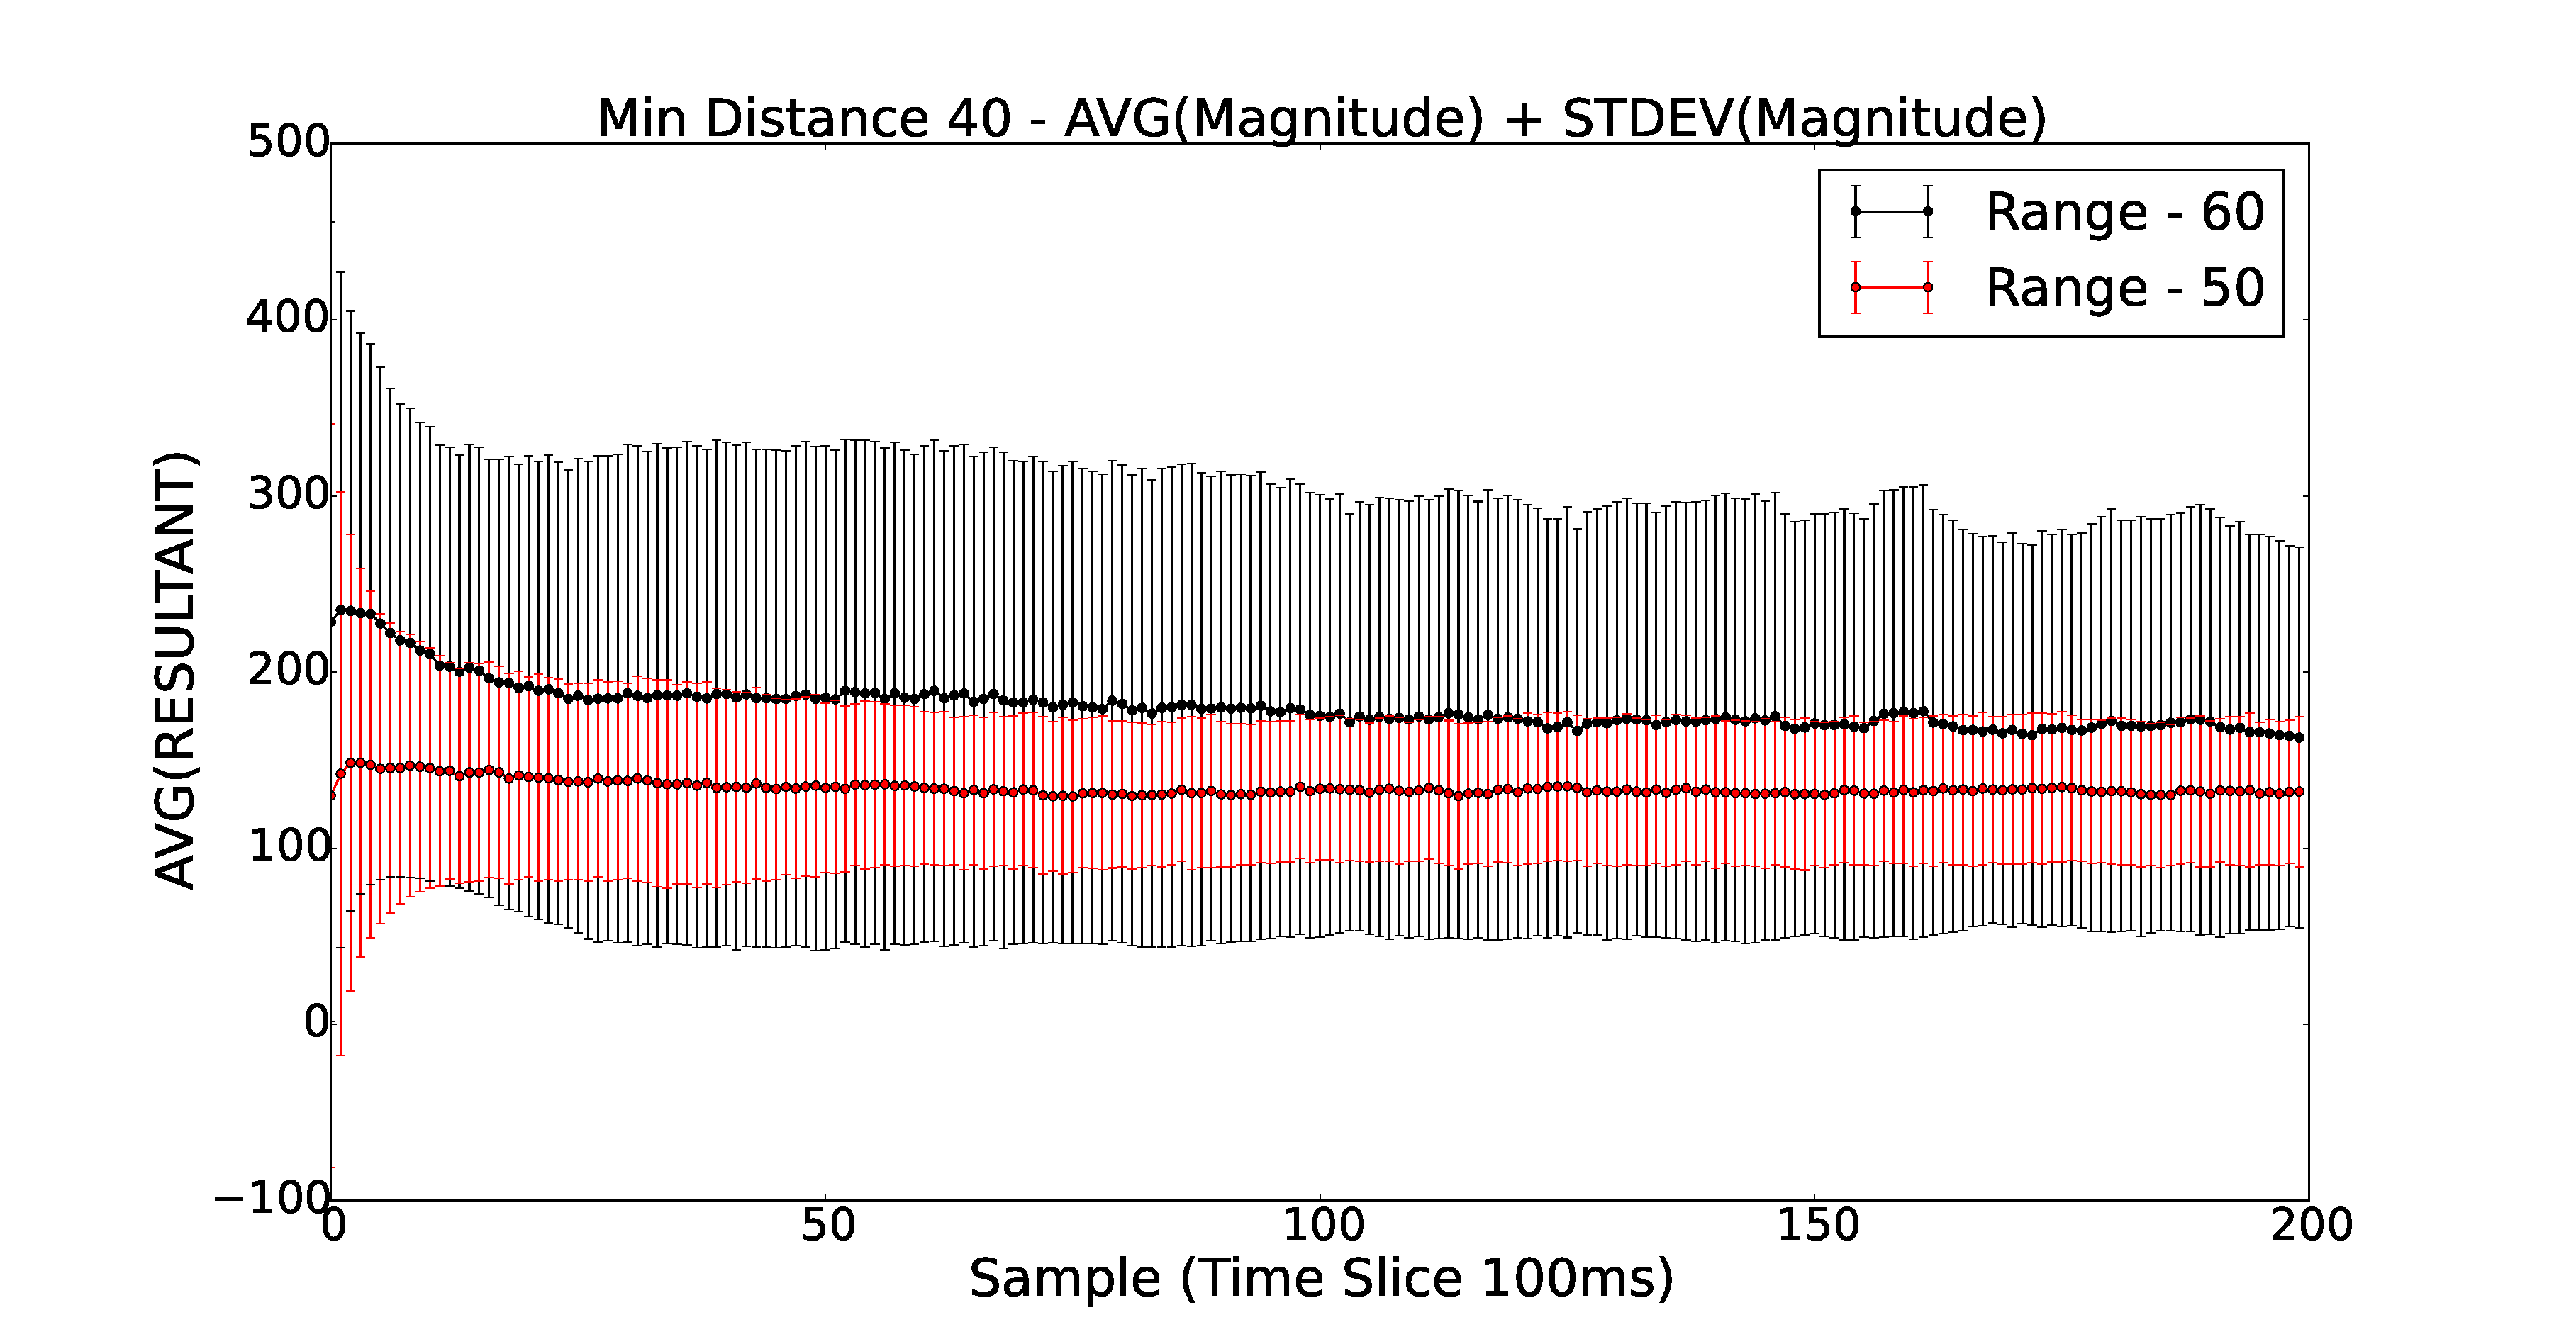
\includegraphics[width=9cm]{figures/StabilityMagnitudeSwarm40-5060}
\end{center}
\caption{Magnitude based \stability{}\label{methods:StabilityMagnitudeSwarm40-5060}}
\end{figure}

A well structured and balanced swarm should therefore have a very low standard deviation in terms of the resultant metric.

\begin{figure}[H]
\begin{center}
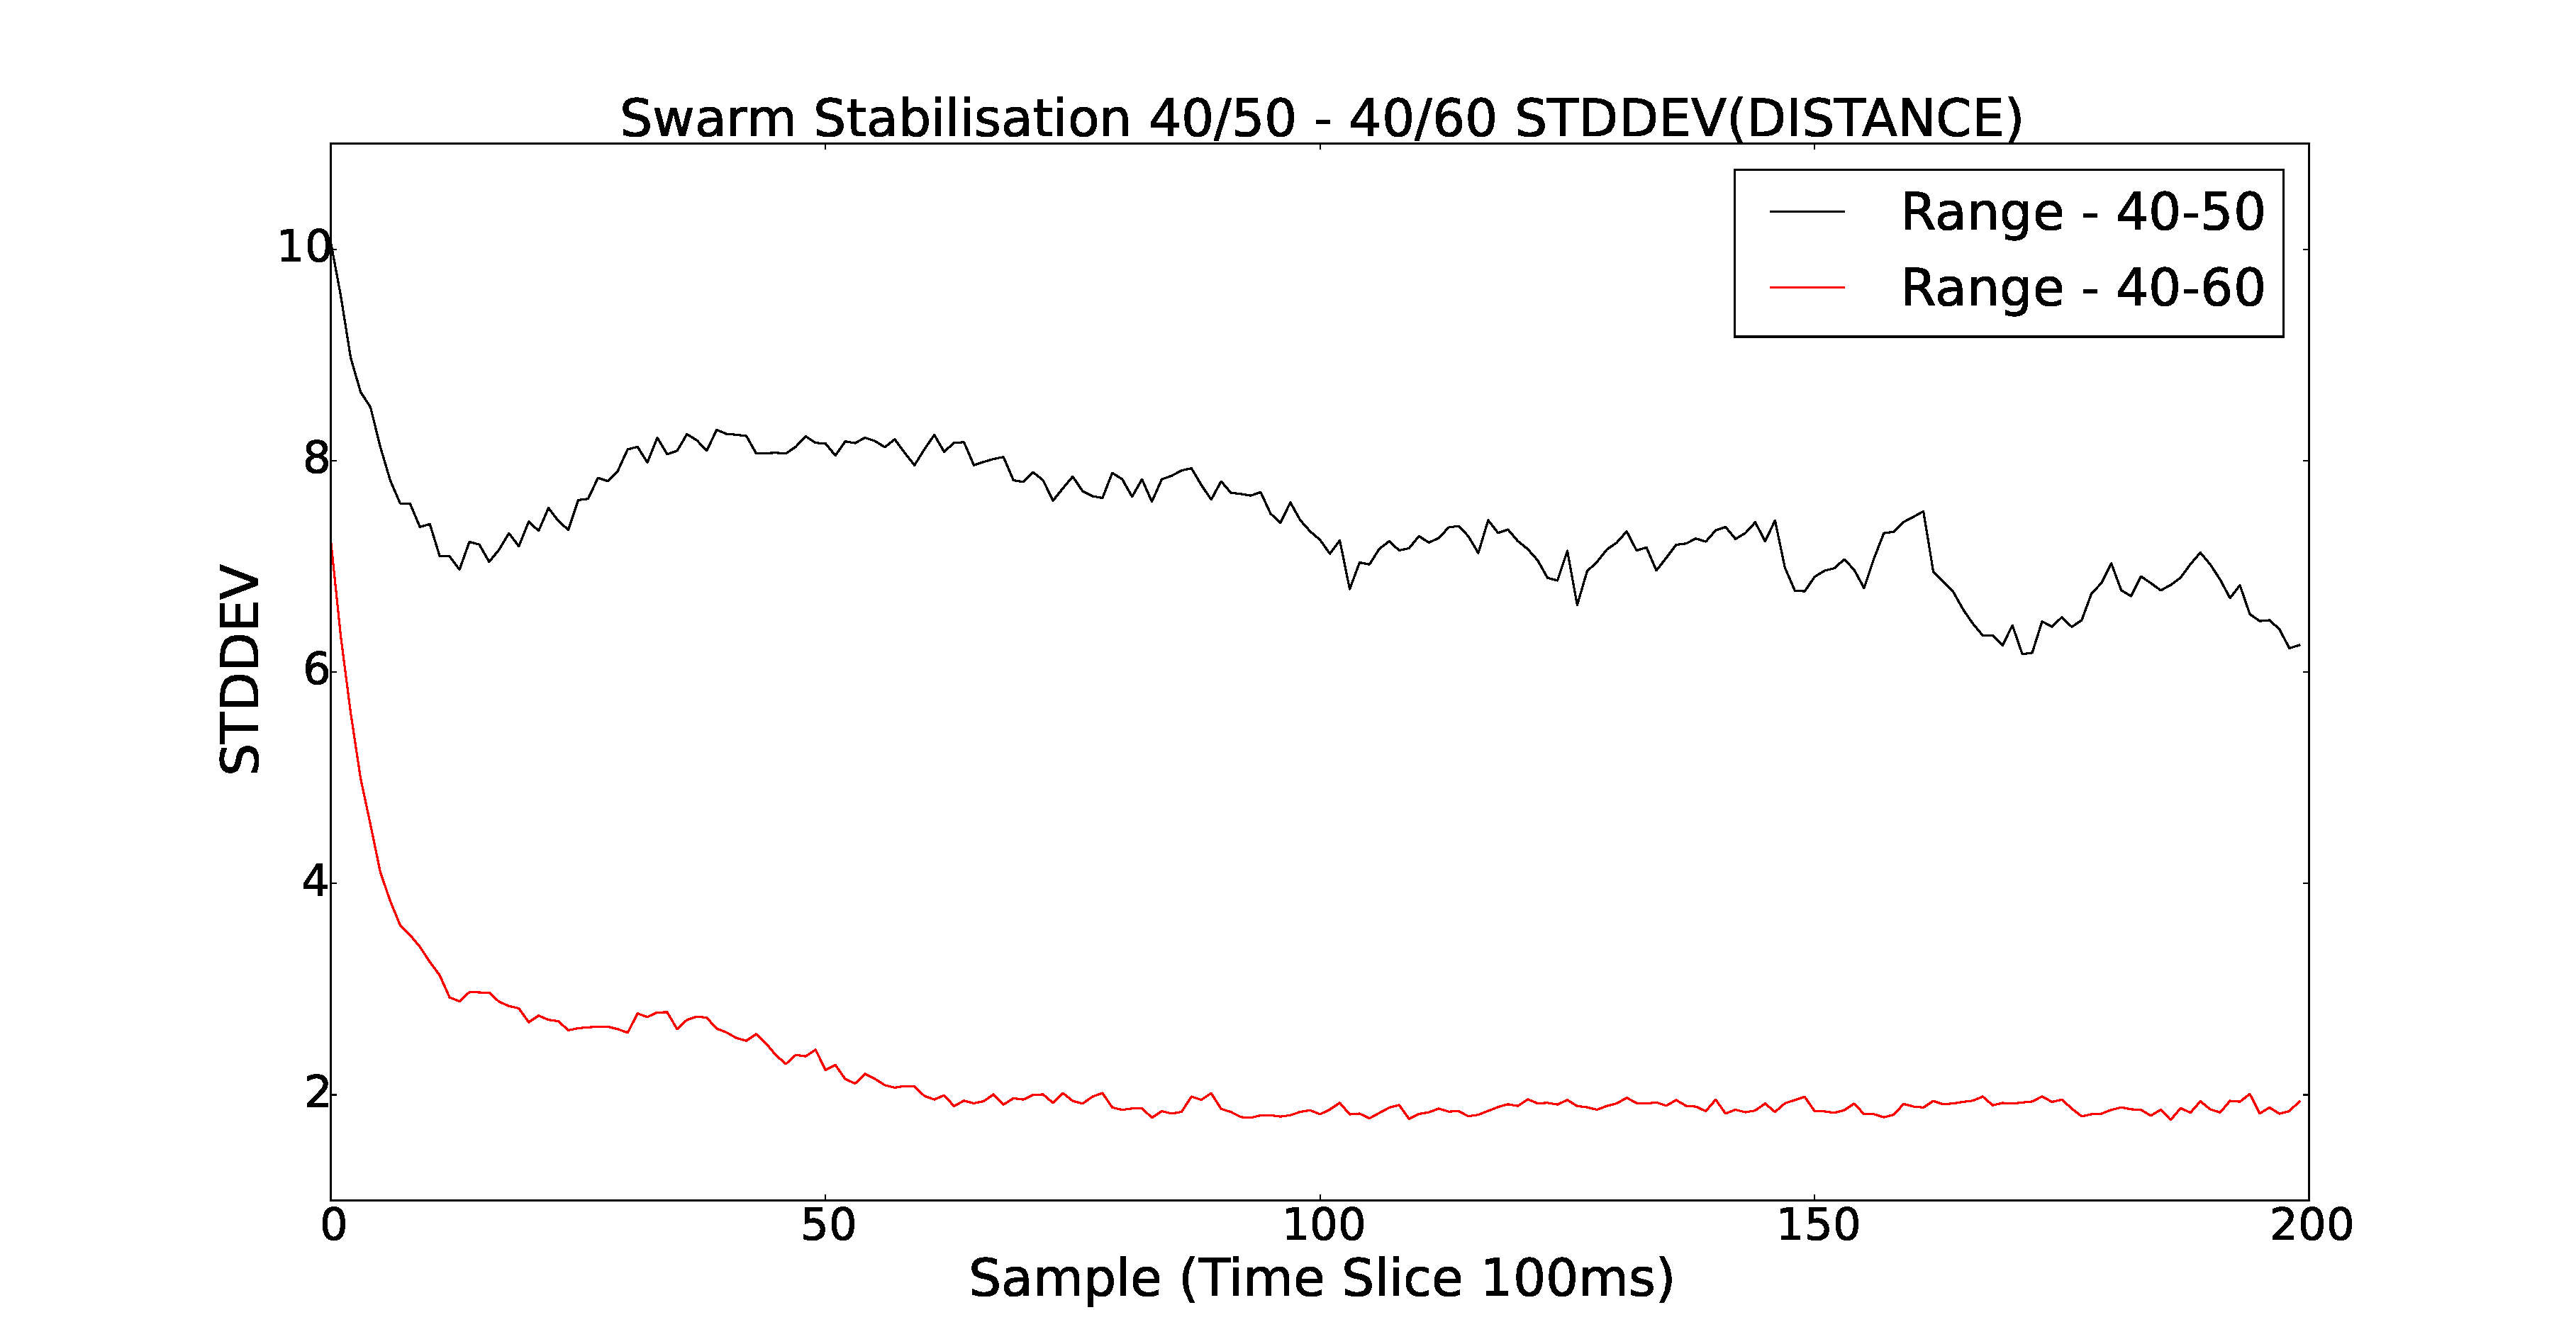
\includegraphics[width=9cm]{figures/StabilityDistanceSwarm}
\end{center}
\caption{Distances based \stability{}\label{methods:StabilityDistanceSwarm}}
\end{figure}

\begin{figure}[H]
\begin{center}
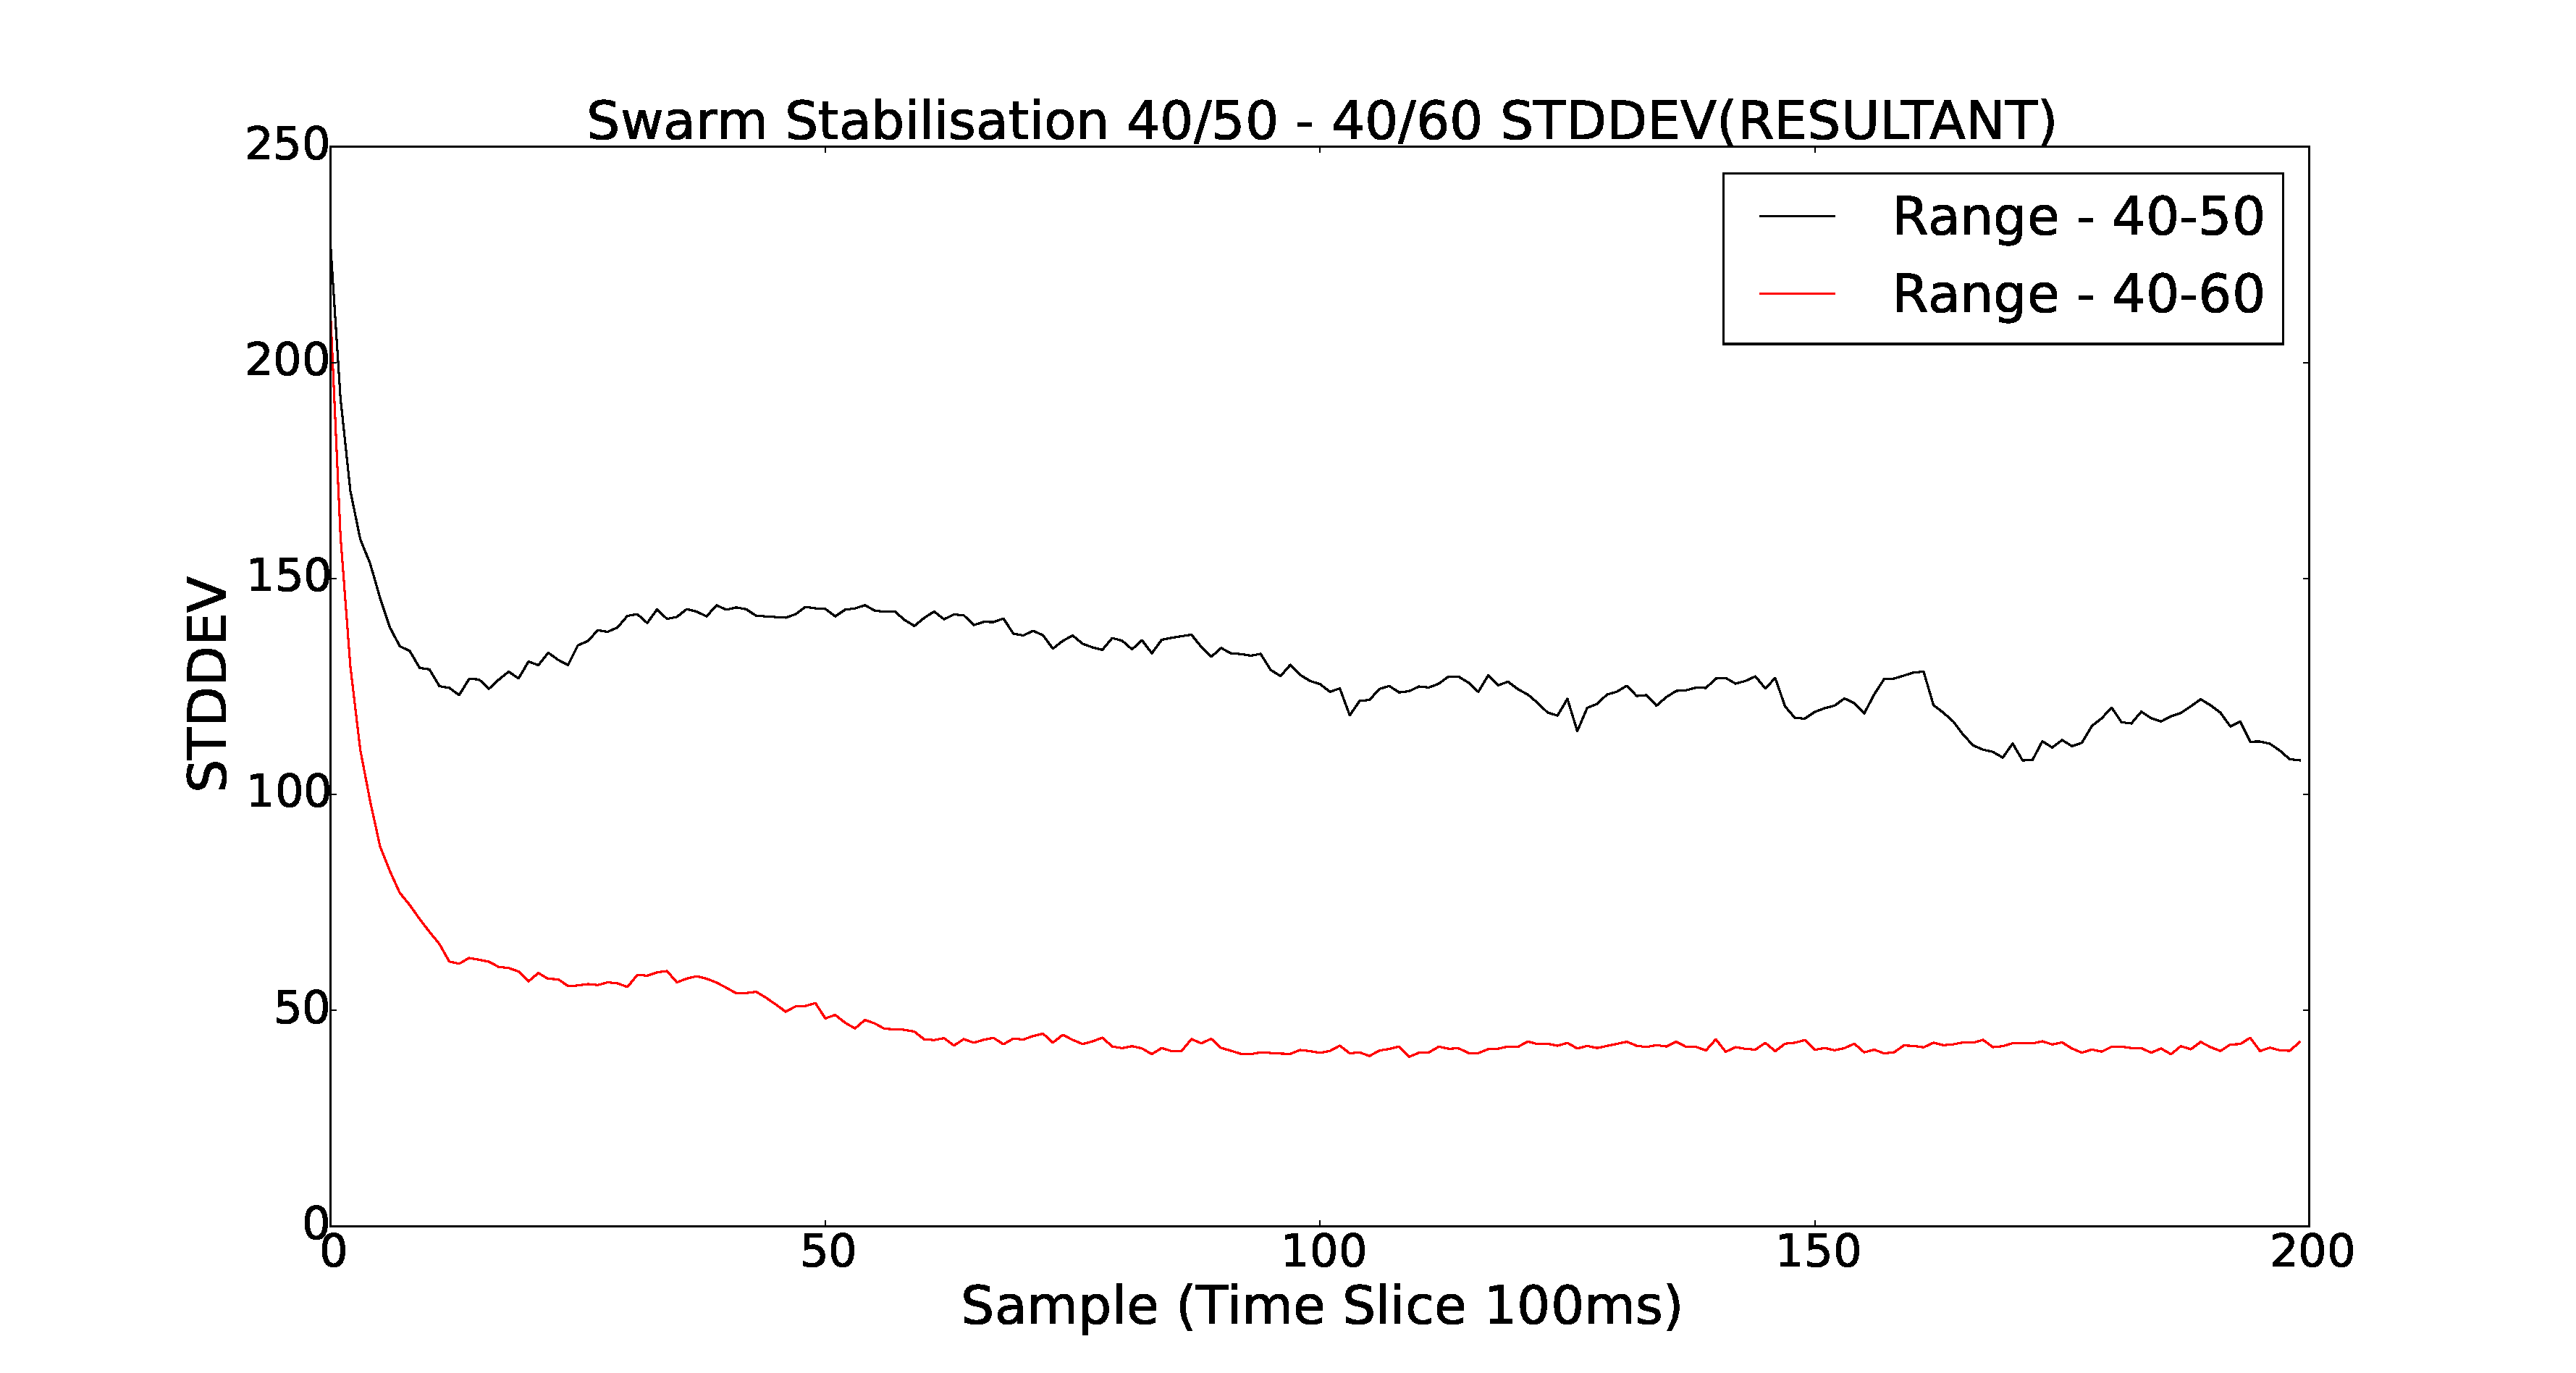
\includegraphics[width=9cm]{figures/StabilityMagnitudeSwarm}
\end{center}
\caption{Magnitude based \stability{}\label{methods:StabilityMagnitudeSwarm}}
\end{figure}

\section{Conclusion and future work\label{section:futureWork}}

The above results show that that the metric created to measure the \stability{} by analysing either the resultant magnitudes or the distance variations that are created within a swarm by the structural methodology used based upon the cohesion and repulsion, it is possible to measure the resulting stability of the swarm.

Use of the stability metrics can be applied to additional scenarios to allow a comparison of the change in \stability{} that a coordination algorithm creates. This could be the addition of a directional bias based on full perimeter detection, partial perimeter detection and all bots having directional capabilities (\Fig{}~\ref{methods:StabilityDistanceSwarmDirection}).
All these scenarios can be combined with object traversal to identify the \stability{} and therefore measure the possible energy efficiency of the algorithms when applied to a specific task such as search and rescue. i.e.~${k_d > 0}$

The graphs below show the effect of taking the swarms used within this paper and applying a directional vector to the swarm ($k_d = 5$), the result is that due to the bots being in constant motion the directional bias of the swarm increases the stability of the swarm this can be seen from the reduced standard deviation, however there are several methods for applying the directional bias and each will effect the overall stability differently. i.e. full perimeter detection, partial perimeter detection and full swarm bias.

\begin{figure}[H]
\begin{center}
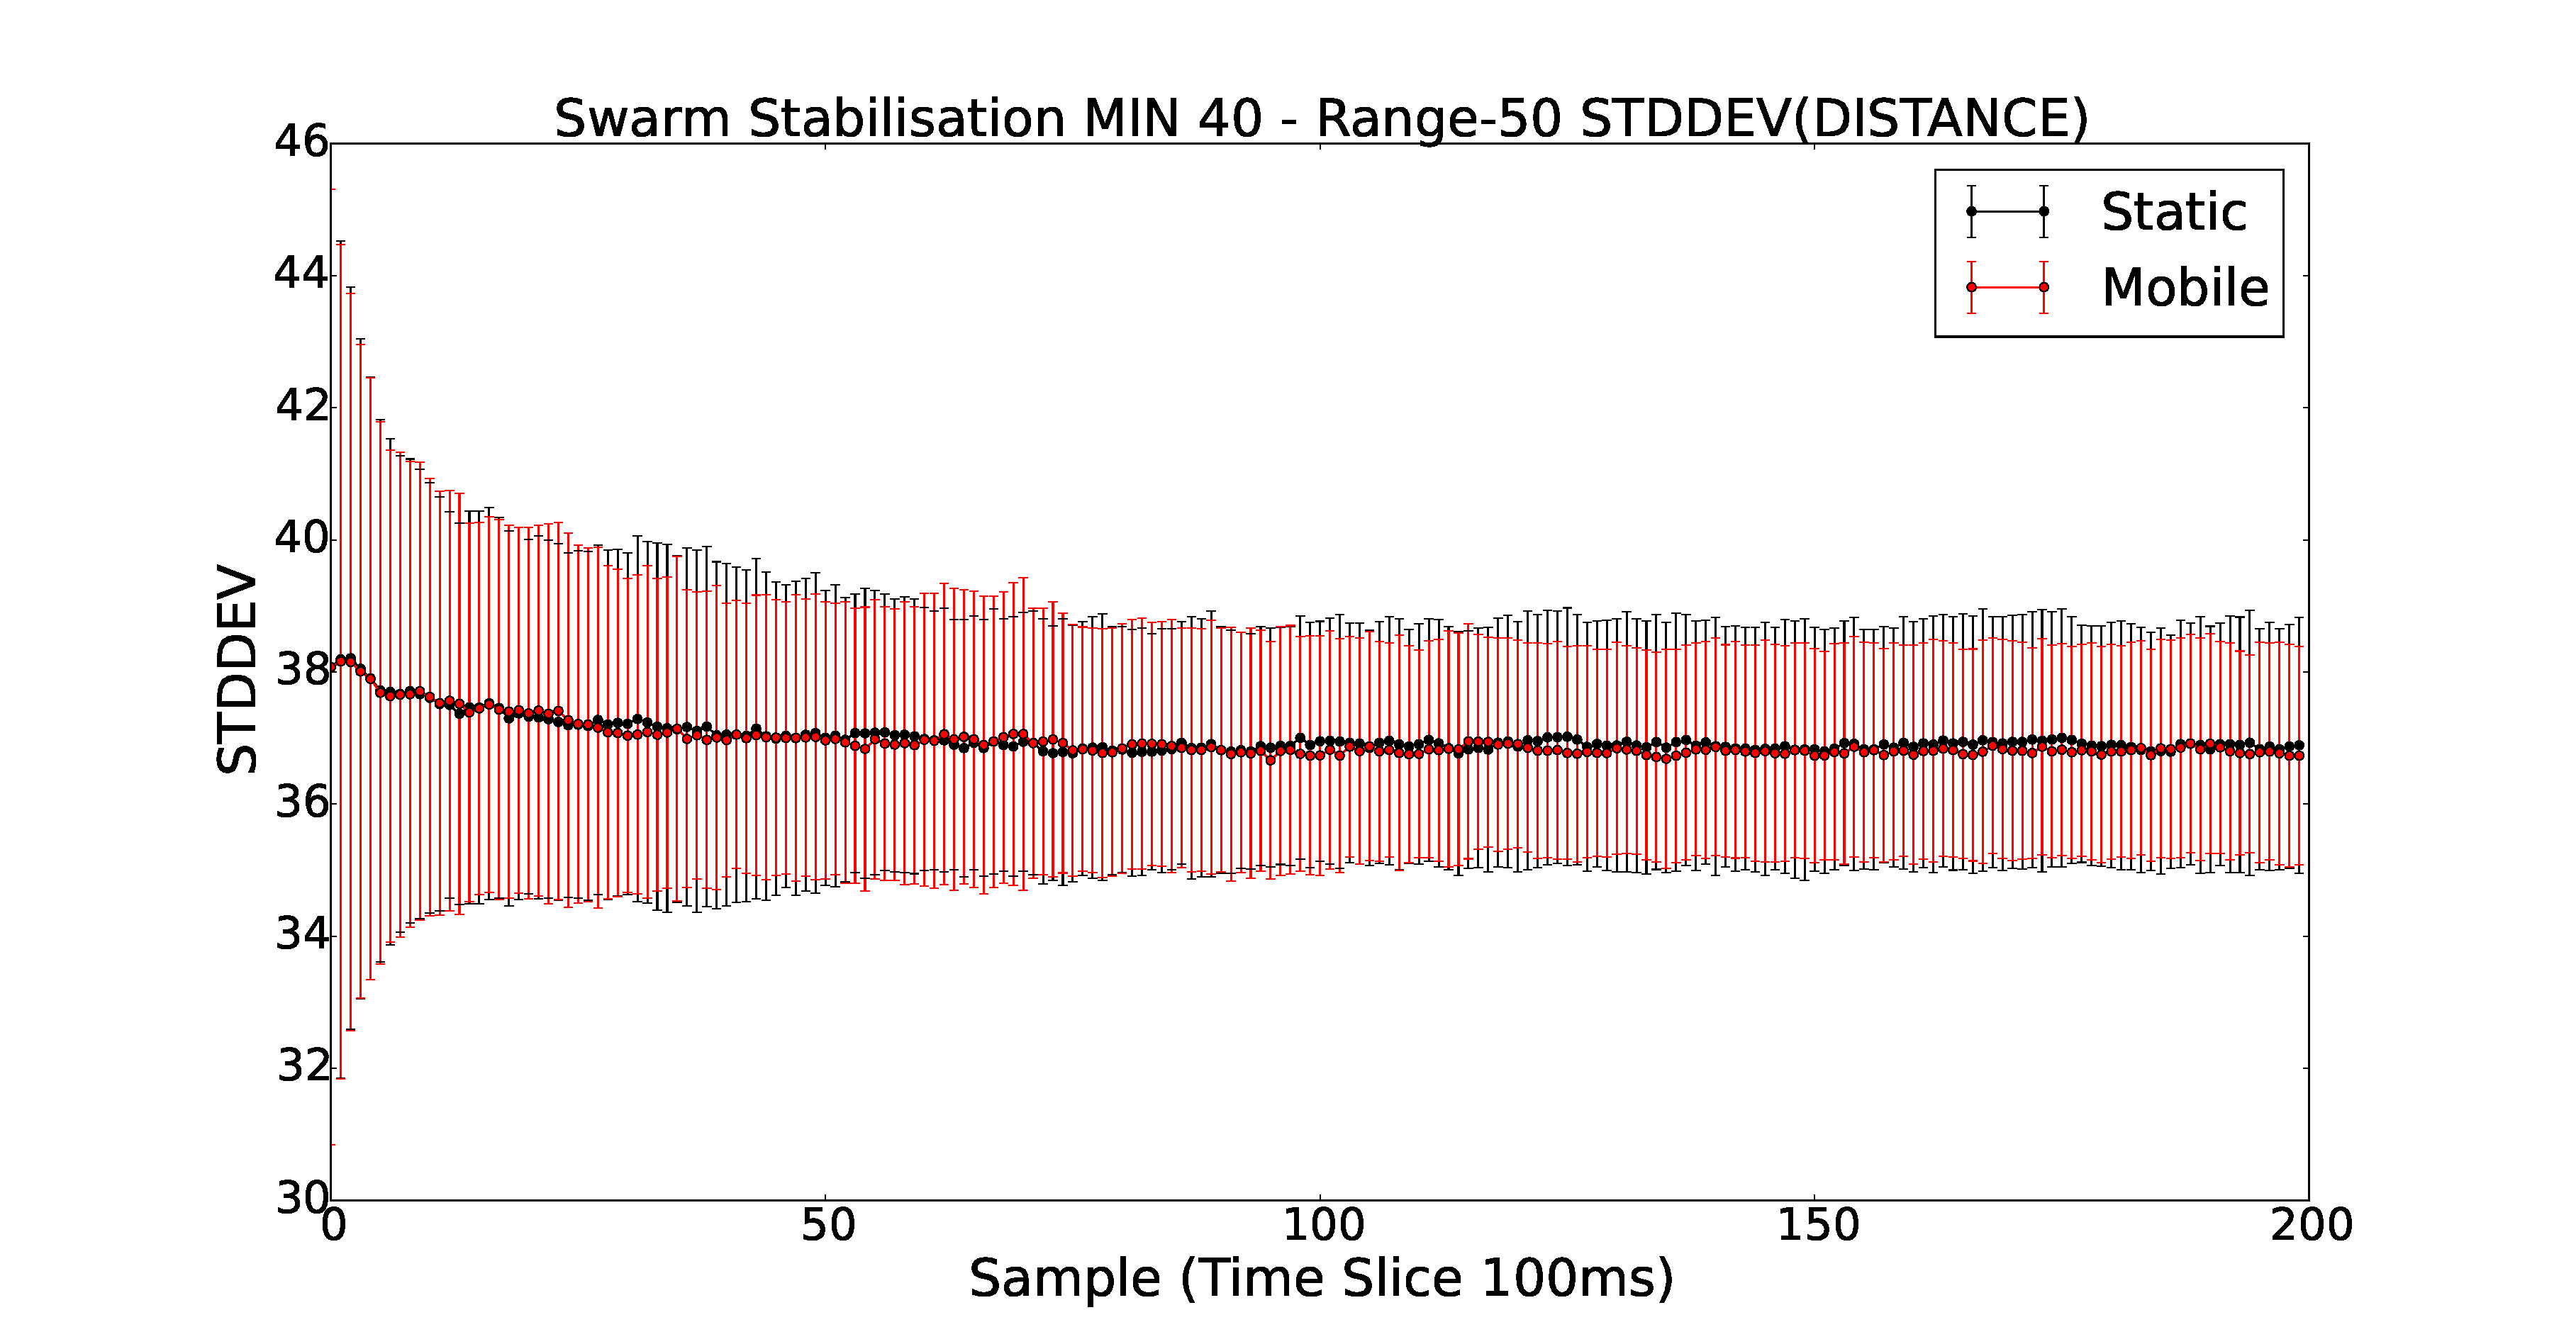
\includegraphics[width=9cm]{figures/StabilityDistanceSwarmDirection}
\end{center}
\caption{Directional \stability{}\label{methods:StabilityDistanceSwarmDirection}}
\end{figure}

\begin{figure}[H]
\begin{center}
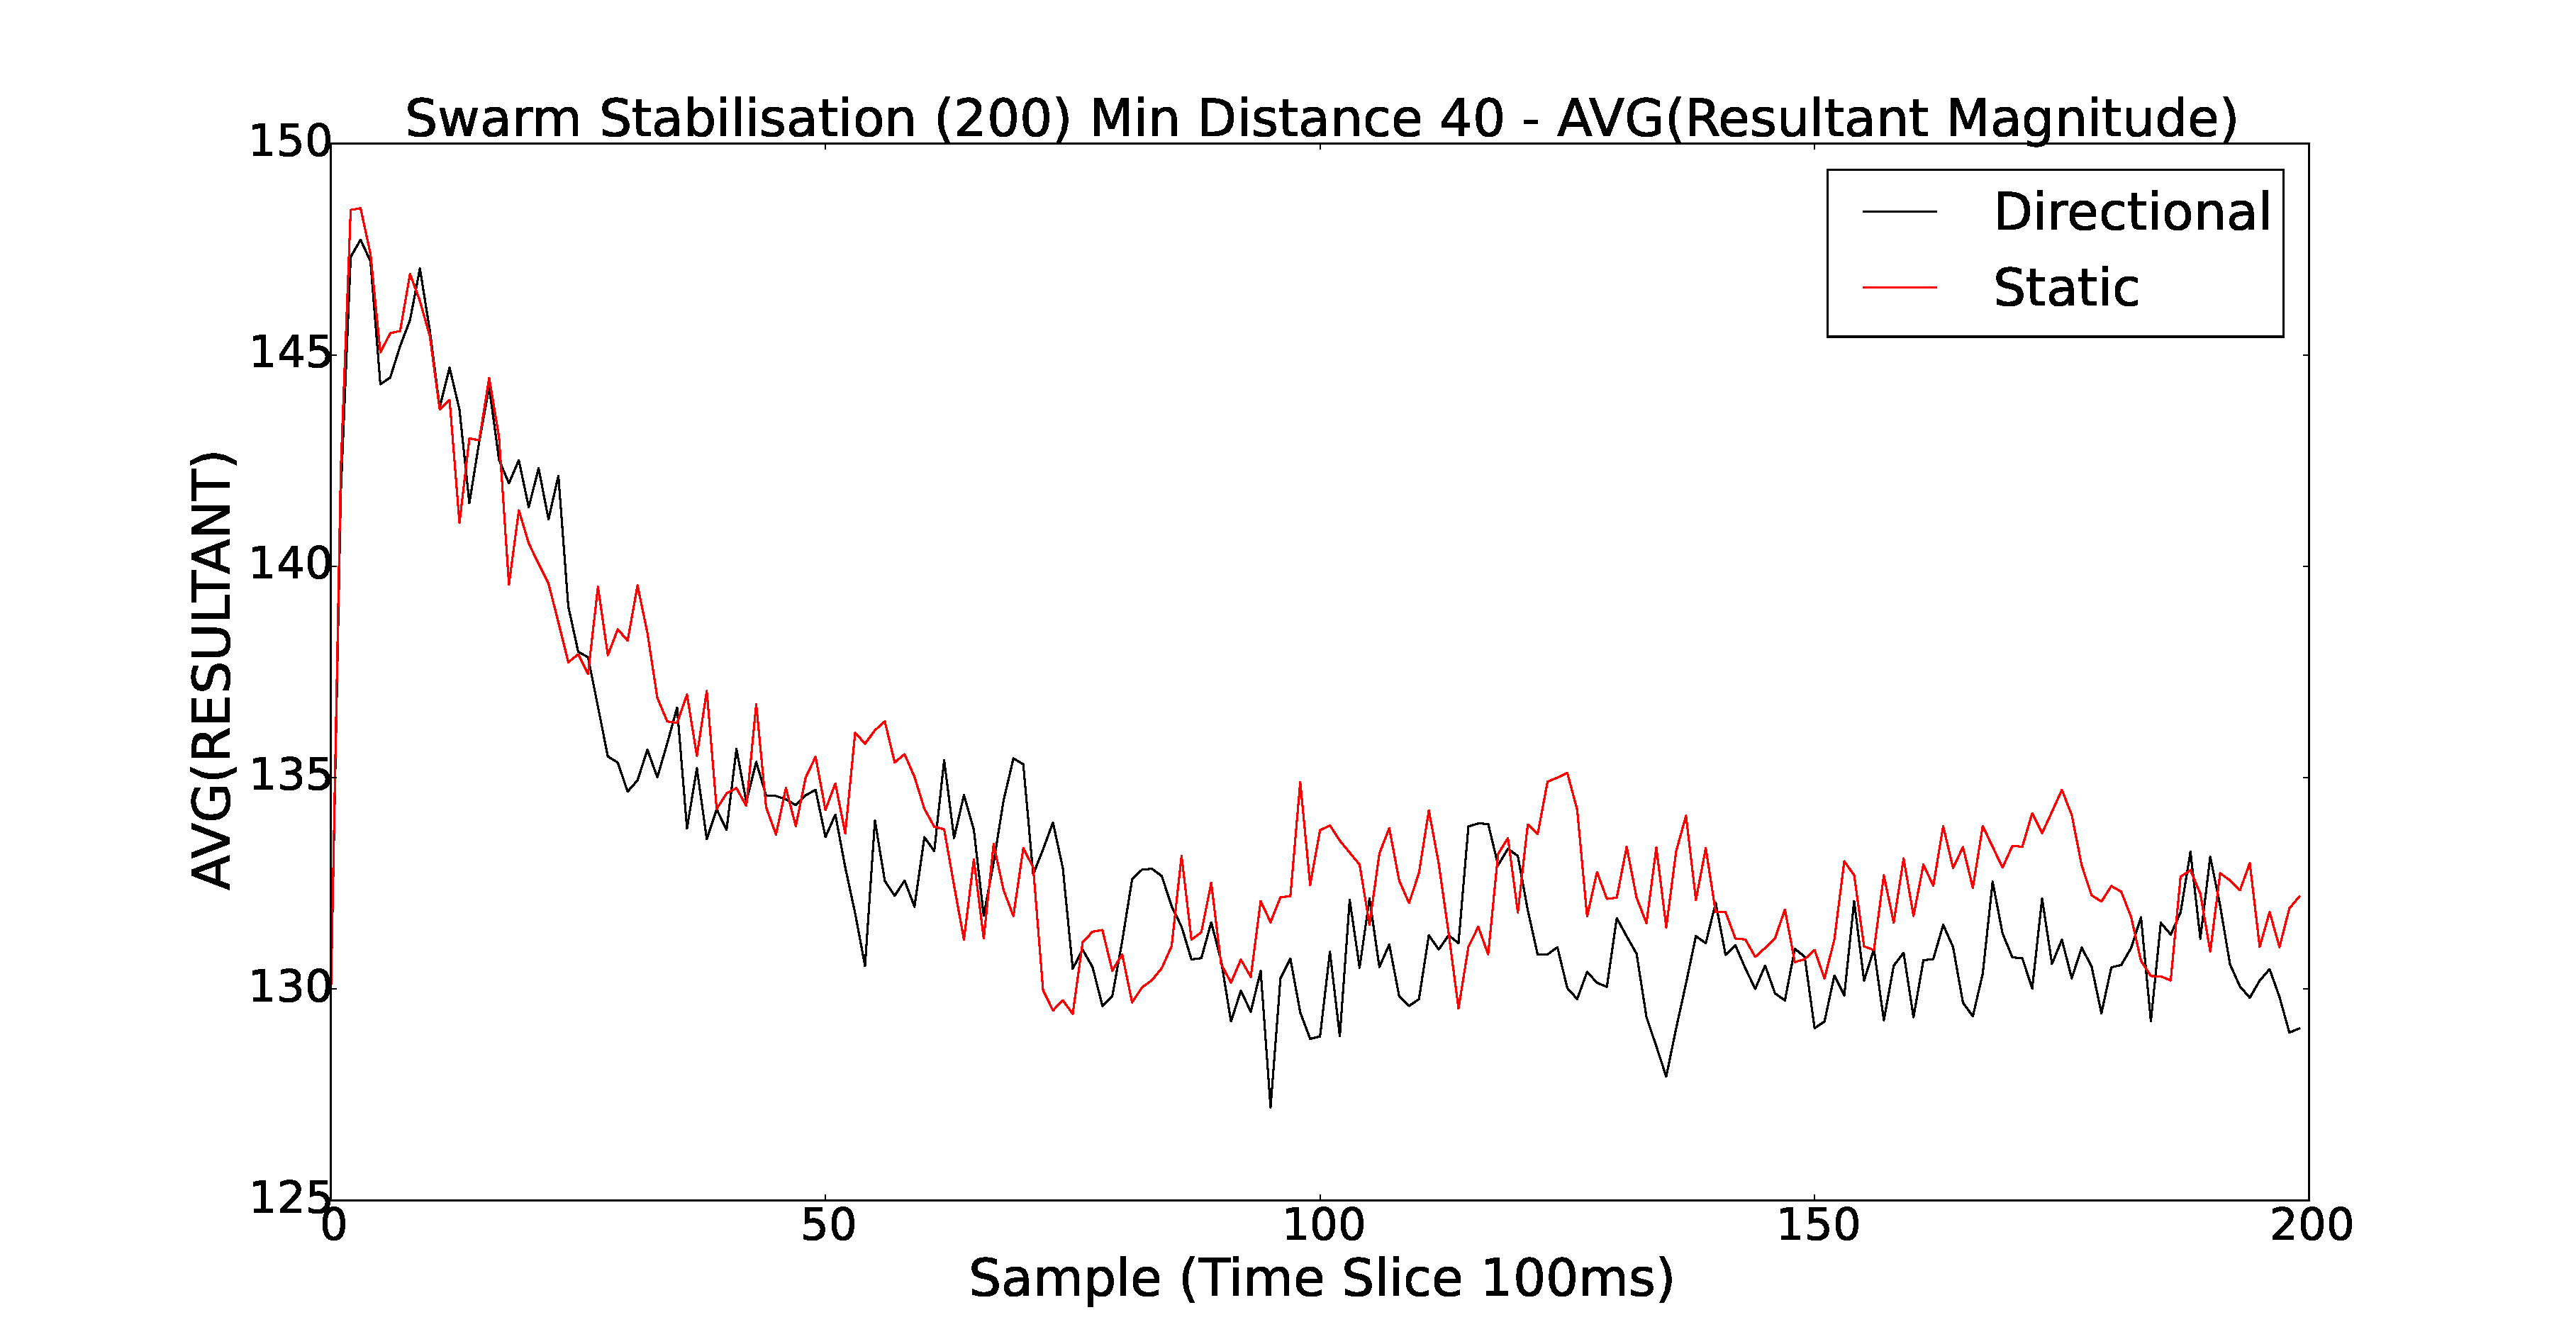
\includegraphics[width=9cm]{figures/StabilityDistanceSwarmDirectionAVGMAG}
\end{center}
\caption{Resultant Magnitude \stability{}\label{methods:StabilityDistanceSwarmDirectionAVGMAG}}
\end{figure}


\bibliographystyle{plain}
\bibliography{stability}

\end{document}
